\section{LABORATORIOS CON SOFTWARE Y HARDWARE}
\begin{frame}

\pgfdeclareimage[width=\paperwidth,height=\paperheight]{bg}{imagenes/fondo_seccion}
\setbeamertemplate{background}{\pgfuseimage{bg}}

\definecolor{greenU}{RGB}{212,202,72}
\setbeamercolor{block body}{fg=Black,bg=greenU}
\begin{block}{}
\centering
\vspace{8mm}
\Large{LABORATORIOS CON SOFTWARE Y HARDWARE}
\vspace{8mm}
\end{block}
\end{frame}
%-----------------------

{
\begin{frame}
\frametitle{Parte III - Tabla de contenidos}
\begin{spacing}{1.5}
\tableofcontents[currentsection,sectionstyle=hide/hide,subsectionstyle=show/show/hide, subsubsectionstyle=hide]
\end{spacing}
\end{frame}
}


\subsection{Lab8: Receptor FM monofónico}
%*********************
\begin{frame}{}

\pgfdeclareimage[width=\paperwidth,height=\paperheight]{bg}{imagenes/fondo_lab}
\setbeamertemplate{background}{\pgfuseimage{bg}}

\bfseries{\textrm{\LARGE Lab8\\ \Large Receptor FM monofónico}}
\raggedright
\end{frame}
%*********************



\begin{frame}{Receptor FM monofónico}

\pgfdeclareimage[width=\paperwidth,height=\paperheight]{bg}{imagenes/fondo3}
\setbeamertemplate{background}{\pgfuseimage{bg}}


En este laboratorio, se realizará la simulación de un receptor FM monofónico en el cual se muestra la función de cada uno de los bloques que conforma dicho receptor, además se muestra el proceso matemático para llegar a 48 KHz de la tasa de muestreo que se va a establecer.



\end{frame}
%---------------------------------

\begin{frame}{Modulación de frecuencia}

Se refiere a la forma de transmitir información a través de una Onda portadora variando su frecuencia. En este tipo de modulación la variación se produce en los saltos de frecuencias. \\ \vspace{2mm}

La modulación de frecuencia se usa comúnmente en las radiofrecuencias de muy alta frecuencia por la alta fidelidad de la radiodifusión de la música y el habla. El sonido de la televisión analógica también se difunde por medio de FM. \\ \vspace{2mm}

La modulación de frecuencia también se utiliza en las frecuencias de audio para sintetizar sonido. Está técnica, conocida como síntesis FM, fue popularizada a principios de los sintetizadores digitales y se convirtió en una característica estándar para varias generaciones de tarjetas de sonido de computadoras personales.

\end{frame}
%---------------------------------


\begin{frame}{Modulación de frecuencia}

\textbf{Aplicaciones en radio}

Dentro de las aplicaciones de FM se encuentra la radio, donde los receptores emplean un detector de FM y el sintonizador es capaz de recibir la señal más fuerte de las que transmiten en la misma frecuencia. Otra de las características que presenta FM es la de poder transmitir señales estereofónicas. \\ \vspace{2mm}

\textbf{Otras aplicaciones}

Entre otras de sus aplicaciones se encuentran la televisión, SECAM: El sistema de televisión en color SECAM modula la información de color en FM. como sub-portadora de sonido; en micrófonos inalámbricos; y como ayuda en navegación aérea, En los sistemas de vídeo analógicos, incluyendo VHS, para registrar la luminancia (blanco y negro) de la señal de video\cite{Wikipedia8}.\\ \vspace{2mm}


\end{frame}
%---------------------------------

\begin{frame}{Diagrama del receptor FM monofónico}

\begin{figure}[H]
\centering
\vspace{-3mm}
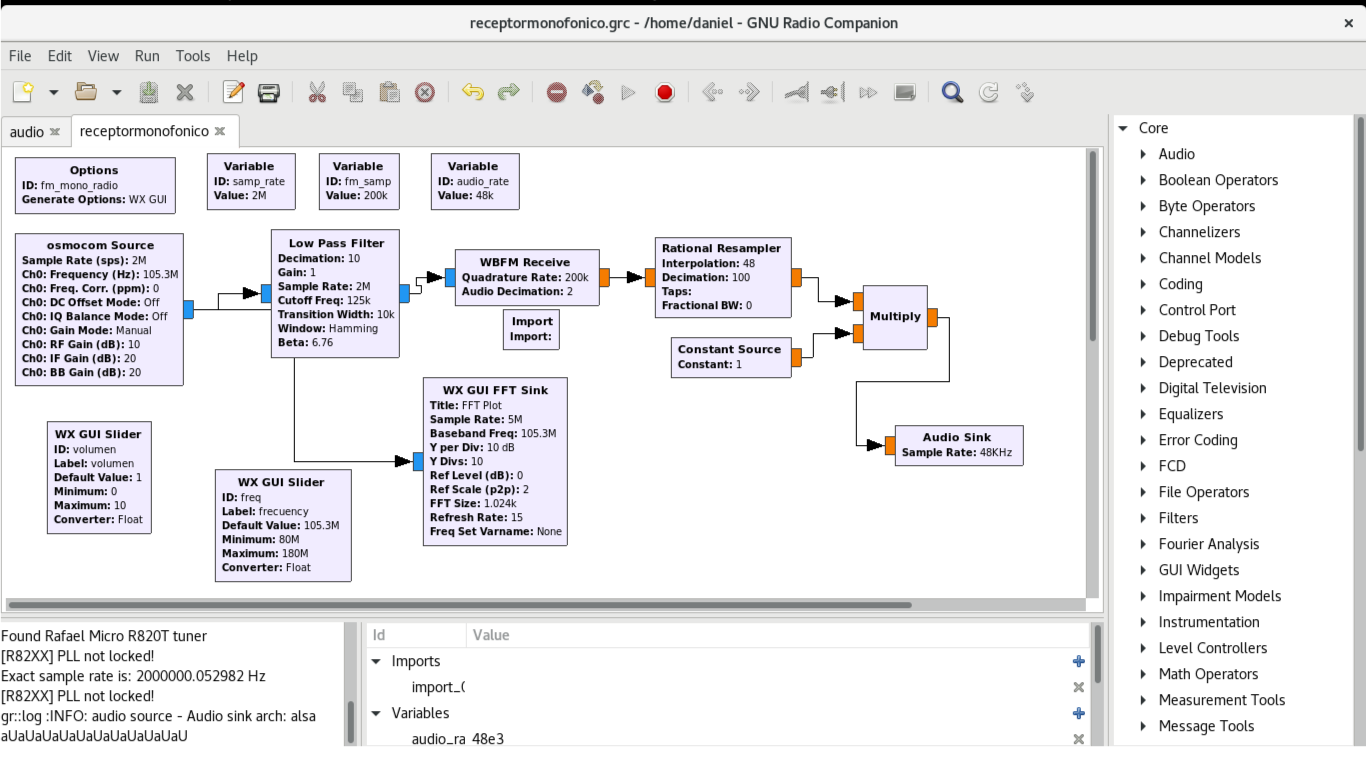
\includegraphics[width=\textwidth]{parte3/lab8/pdf/lab8_1.pdf}
\end{figure}

\end{frame}
%---------------------------------

\begin{frame}{Receptor FM monofónico}

\begin{figure}[H]
\centering
\vspace{-3mm}
\includegraphics[width=\textwidth]{parte3/lab8/pdf/lab8_2.pdf}
\end{figure}

\end{frame}
%---------------------------------

\begin{frame}{Receptor FM monofónico}

\begin{figure}[H]
\centering
\vspace{-3mm}
\includegraphics[width=\textwidth]{parte3/lab8/pdf/lab8_3.pdf}
\end{figure}

\end{frame}
%---------------------------------

\begin{frame}{Receptor FM monofónico}

\begin{figure}[H]
\centering
\vspace{-3mm}
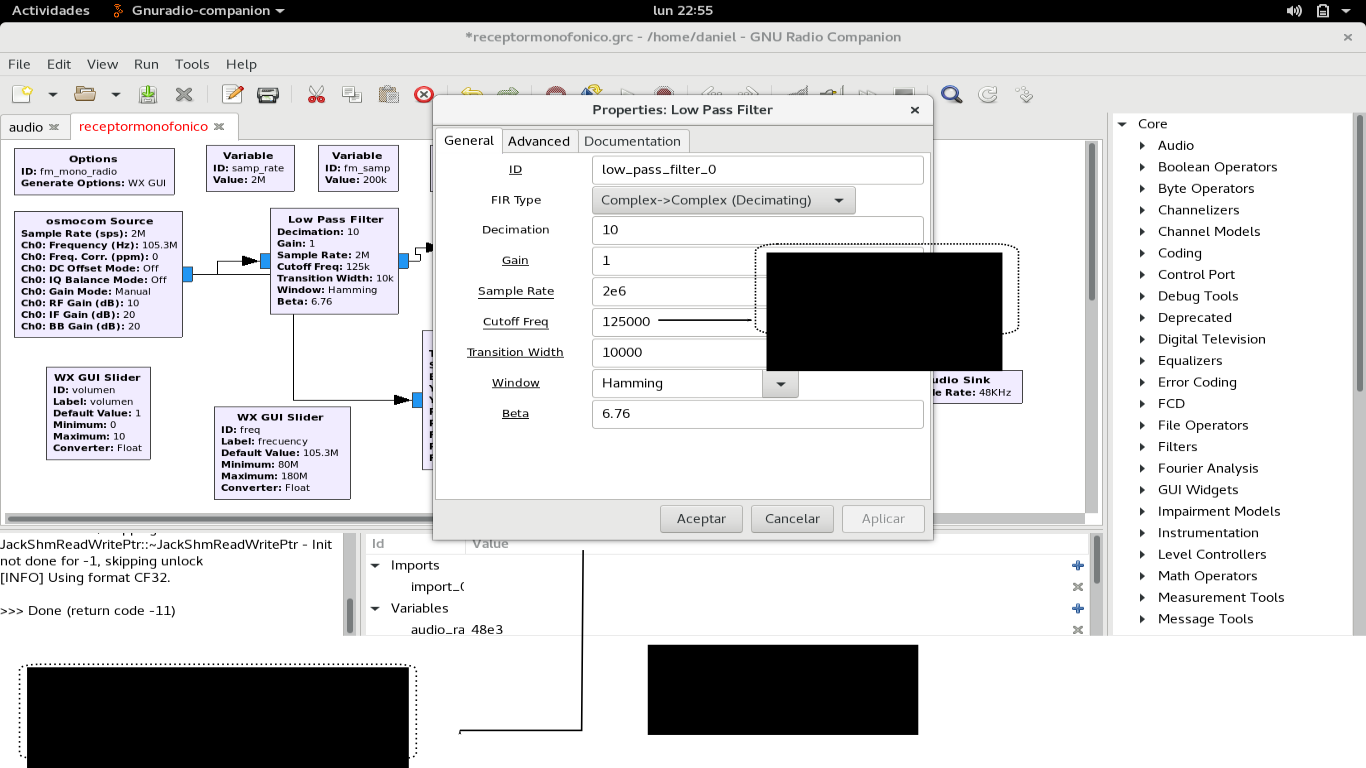
\includegraphics[width=\textwidth]{parte3/lab8/pdf/lab8_4.pdf}
\end{figure}

\end{frame}
%---------------------------------

\begin{frame}{Receptor FM monofónico}

\begin{figure}[H]
\centering
\vspace{-3mm}
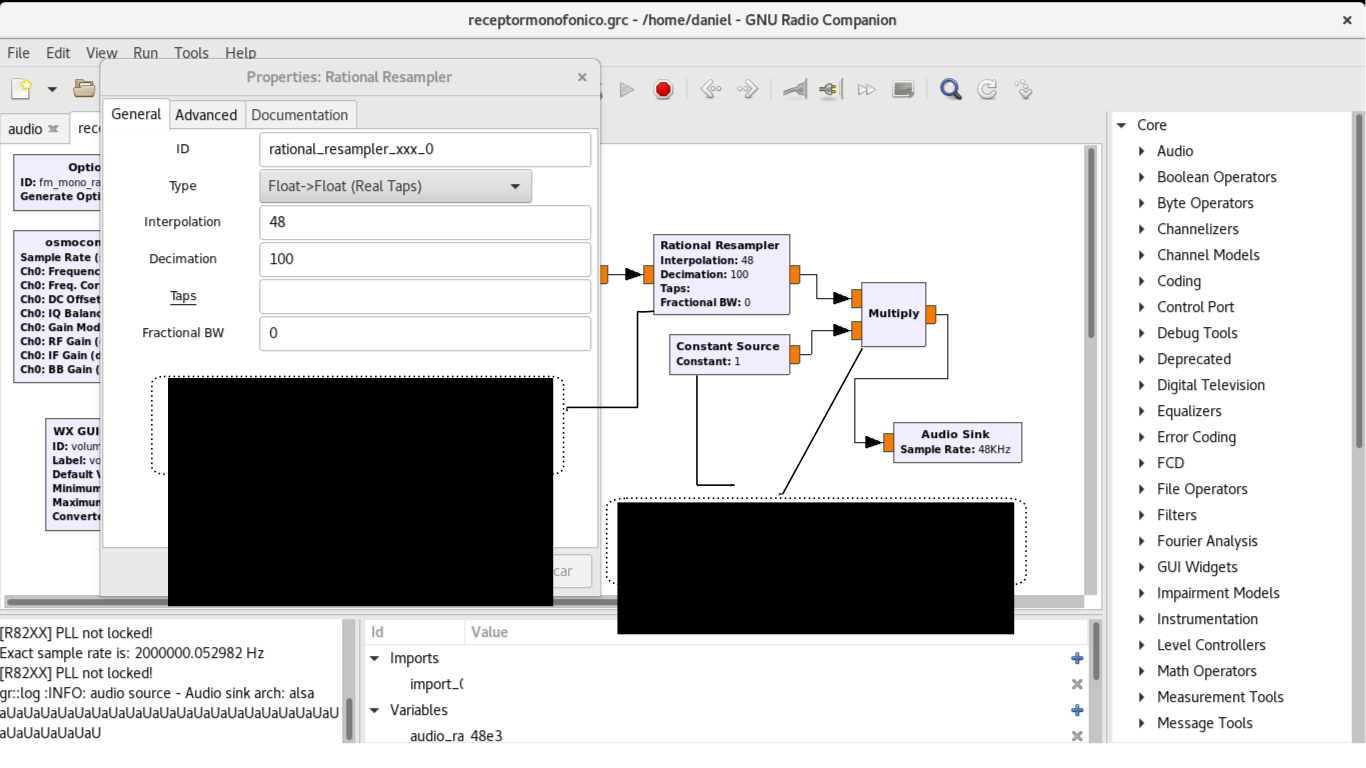
\includegraphics[width=\textwidth]{parte3/lab8/pdf/lab8_5.pdf}
\end{figure}

\end{frame}
%---------------------------------

\begin{frame}{Receptor FM monofónico}

\begin{figure}[H]
\centering
\vspace{-3mm}
\includegraphics[width=\textwidth]{parte3/lab8/pdf/lab8_6.pdf}
\end{figure}

\end{frame}
%---------------------------------

\begin{frame}{Proceso matemático}

\begin{figure}[H]
\centering
\vspace{-3mm}
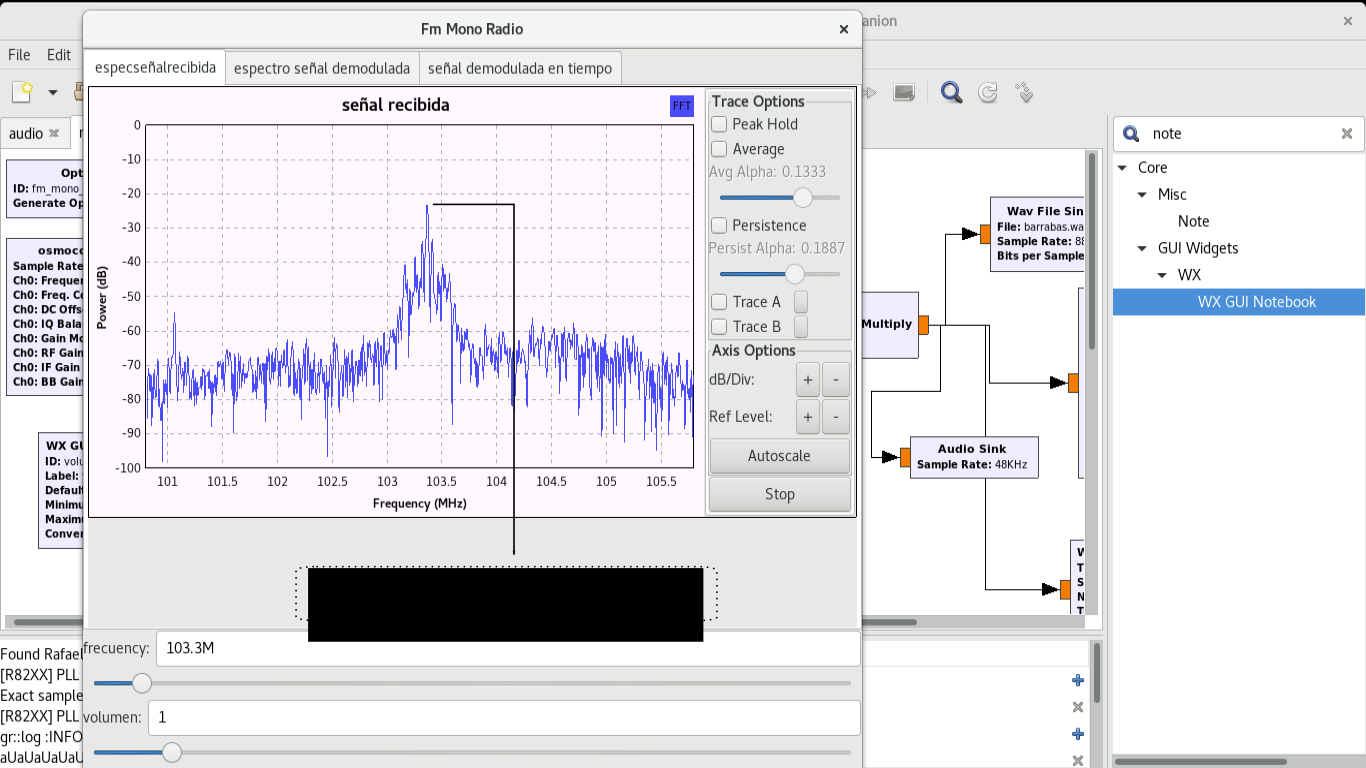
\includegraphics[width=\textwidth]{parte3/lab8/pdf/lab8_7.pdf}
\end{figure}

\end{frame}
%---------------------------------

\begin{frame}{Receptor FM monofónico}

\begin{figure}[H]
\centering
\vspace{-3mm}
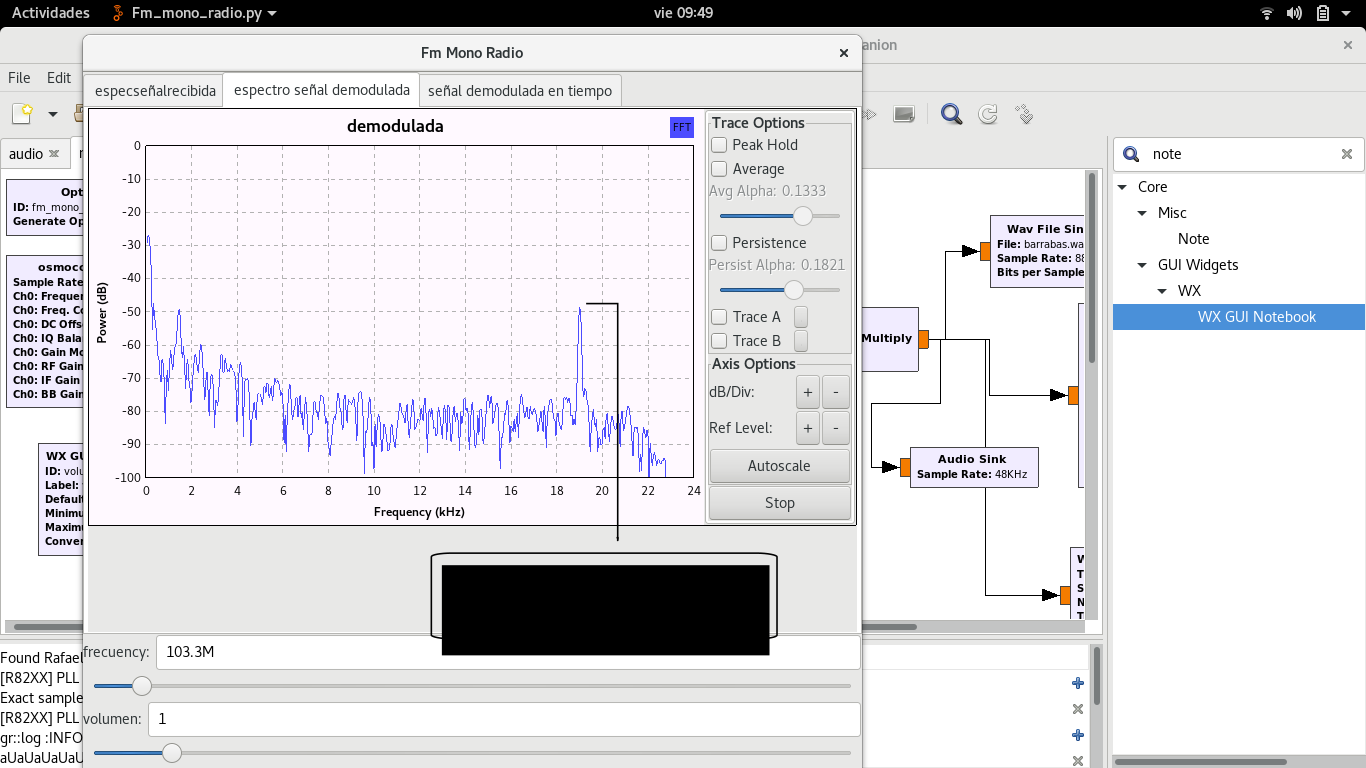
\includegraphics[width=\textwidth]{parte3/lab8/pdf/lab8_8.pdf}
\end{figure}

\end{frame}
%---------------------------------

\begin{frame}{Espectro señal recibida}

\begin{figure}[H]
\centering
\vspace{-3mm}
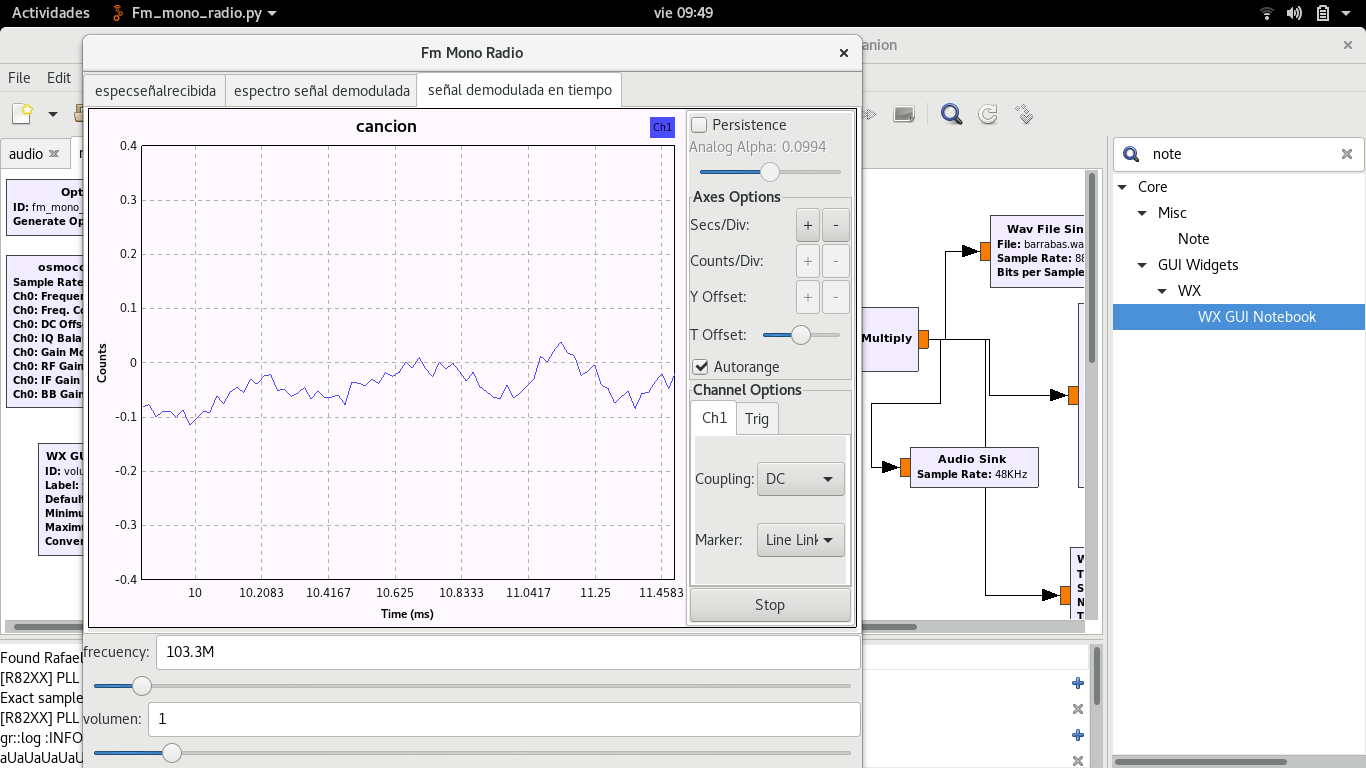
\includegraphics[width=\textwidth]{parte3/lab8/pdf/lab8_9.pdf}
\end{figure}

\end{frame}
%---------------------------------


\begin{frame}{Espectro señal demodulada}

\begin{figure}[H]
\centering
\vspace{-3mm}
\includegraphics[width=\textwidth]{parte3/lab8/pdf/lab8_10.pdf}
\end{figure}

\end{frame}
%---------------------------------


\begin{frame}{Señal demodulada en el tiempo}

\begin{figure}[H]
\centering
\vspace{-3mm}
\includegraphics[width=\textwidth]{parte3/lab8/pdf/lab8_11.pdf}
\end{figure}

\end{frame}
%---------------------------------


%///////////////////////////////////////////////////////////////

\subsection{Lab11: Transmisor FM Mono}

%*********************
\begin{frame}{}

\pgfdeclareimage[width=\paperwidth,height=\paperheight]{bg}{imagenes/fondo_lab}
\setbeamertemplate{background}{\pgfuseimage{bg}}

\bfseries{\textrm{\LARGE Lab11\\ \Large Transmisor FM Monofónico}}
\raggedright
\end{frame}
%*********************

\begin{frame}{Transmisor FM Monofónico}

\pgfdeclareimage[width=\paperwidth,height=\paperheight]{bg}{imagenes/fondo3}
\setbeamertemplate{background}{\pgfuseimage{bg}}

El transmisor FM es un dispositivo electrónico que, mediante una antena, irradia ondas electromagnéticas que contienen (o pueden contener) información, como ocurre en el caso de las señales de radio, televisión, telefonía móvil o cualquier otro tipo de radiocomunicación.\\
\vspace{2mm}
Por medio de la modulación angular se puede hacer que un parámetro de la onda portadora cambie de valor según las variaciones de la señal moduladora, que es la información que se quiere transmitir. \\
\vspace{2mm}
Se utiliza esta modulación porque facilita la propagación de la señal de información, ordena el radio-espectro, disminuye dimensiones de antenas, optimiza el ancho de banda de cada canal, evita interferencias entre canales, y Protege la información de las degradaciones por ruido.


\end{frame}
%---------------------------------
\begin{frame}{Transmisor FM Monofónico}

\begin{figure}[H]
\centering
\vspace{-3mm}
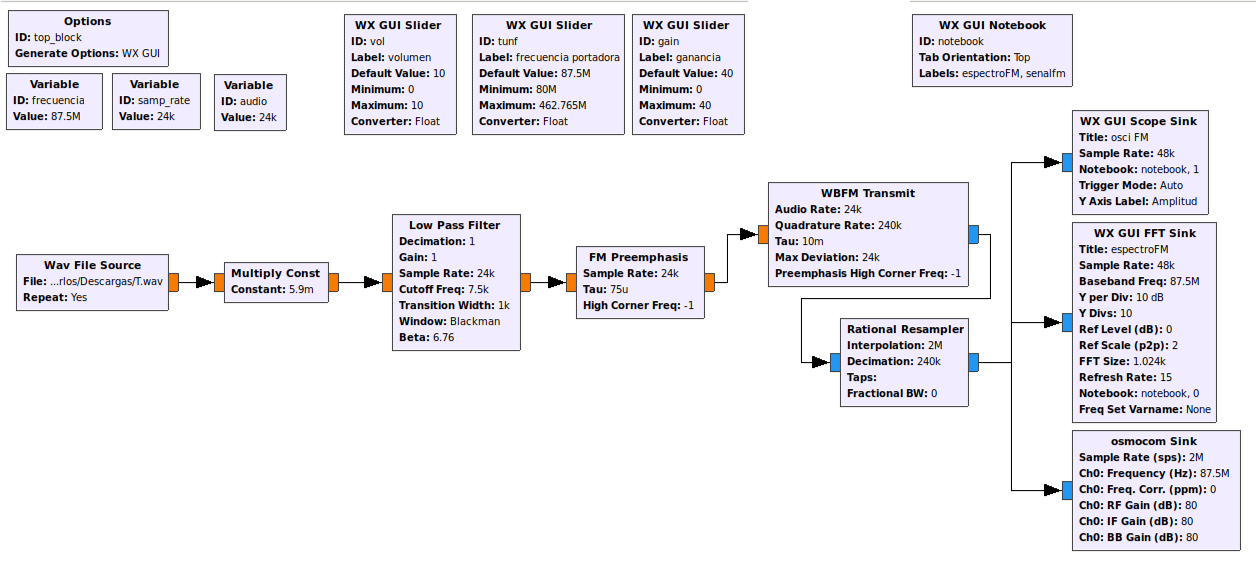
\includegraphics[width=\textwidth]{parte3/lab11/pdf/lab11_1.pdf}
\end{figure}

\end{frame}
%---------------------------------

\begin{frame}{Transmisor FM Monofónico}

\begin{figure}[H]
\centering
\vspace{-3mm}
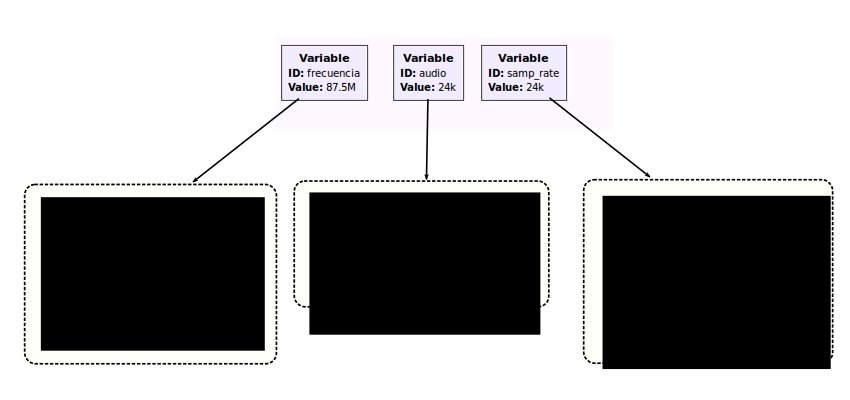
\includegraphics[width=\textwidth]{parte3/lab11/pdf/lab11_2.pdf}
\end{figure}

En este transmisor la fuente es un archivo de audio en formato WAV muestreado a 24 kHz.


\end{frame}
%---------------------------------

\begin{frame}{Transmisor FM Monofónico}

\begin{figure}[H]
\centering
\vspace{-3mm}
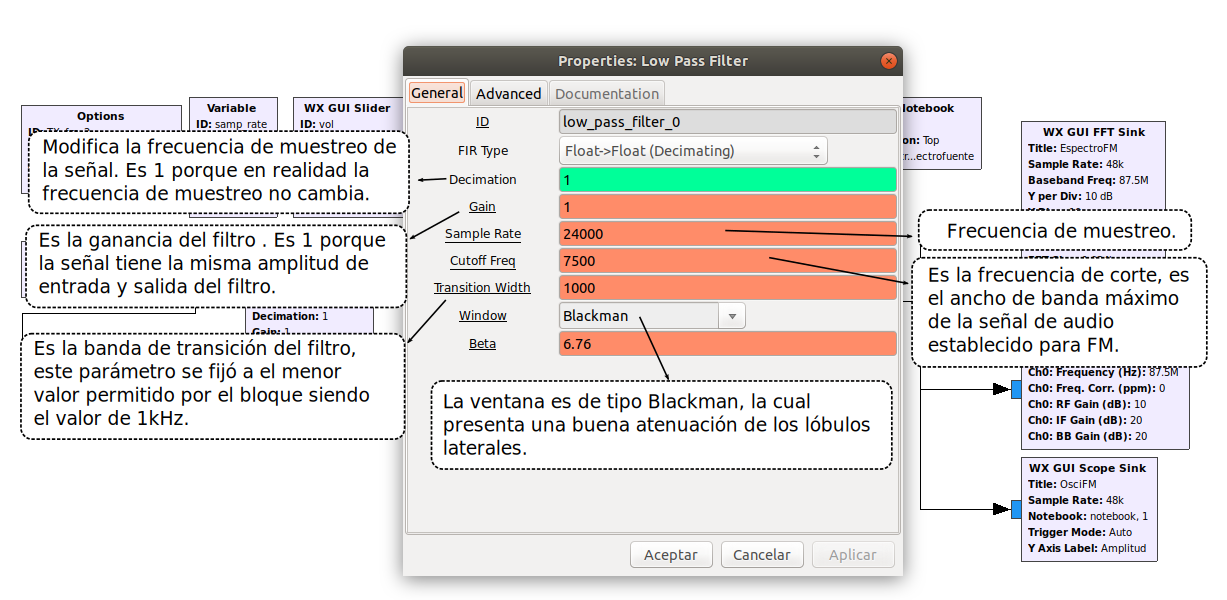
\includegraphics[width=\textwidth]{parte3/lab11/pdf/lab11_3.pdf}
\end{figure}

\end{frame}
%---------------------------------

\begin{frame}{Transmisor FM Monofónico}

\begin{figure}[H]
\centering
\vspace{-3mm}
\includegraphics[width=\textwidth]{parte3/lab11/pdf/lab11_4.pdf}
\end{figure}

\end{frame}
%---------------------------------

\begin{frame}{Transmisor FM Monofónico}

\begin{figure}[H]
\centering
\vspace{-3mm}
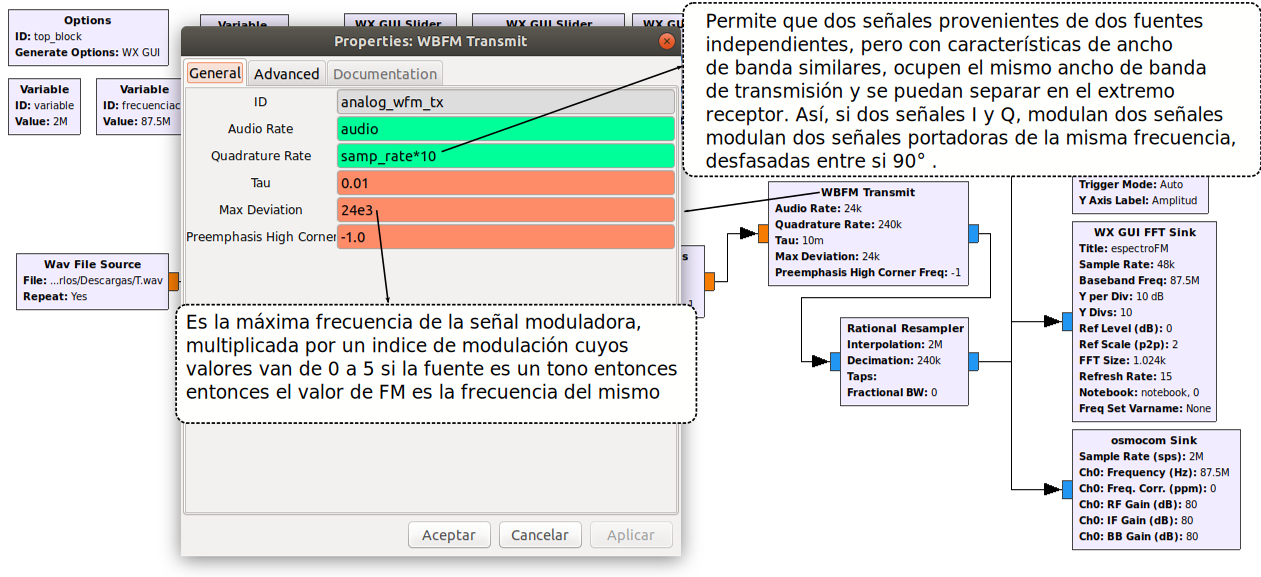
\includegraphics[width=\textwidth]{parte3/lab11/pdf/lab11_5.pdf}
\end{figure}

\end{frame}
%---------------------------------

\begin{frame}{Transmisor FM Monofónico}

\begin{figure}[H]
\centering
\vspace{-3mm}
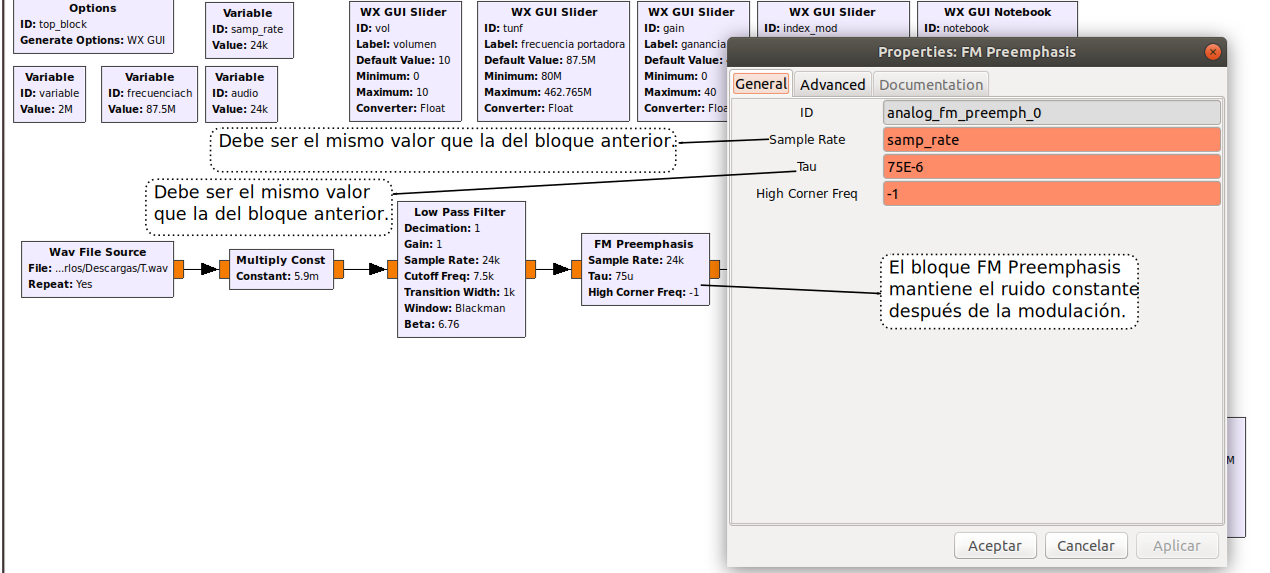
\includegraphics[width=\textwidth]{parte3/lab11/pdf/lab11_6.pdf}
\end{figure}

\end{frame}
%---------------------------------

%///////////////////////////////////////////////////////////////

\subsection{Lab9: Receptor FM Estereo}
%*********************
\begin{frame}{}

\pgfdeclareimage[width=\paperwidth,height=\paperheight]{bg}{imagenes/fondo_lab}
\setbeamertemplate{background}{\pgfuseimage{bg}}

\bfseries{\textrm{\LARGE Lab9\\ \Large Receptor FM Estereofónico}}
\raggedright
\end{frame}
%*********************

\begin{frame}{Receptor FM Estereo}

\pgfdeclareimage[width=\paperwidth,height=\paperheight]{bg}{imagenes/fondo3}
\setbeamertemplate{background}{\pgfuseimage{bg}}

\begin{figure}[H]
\centering
\vspace{-3mm}
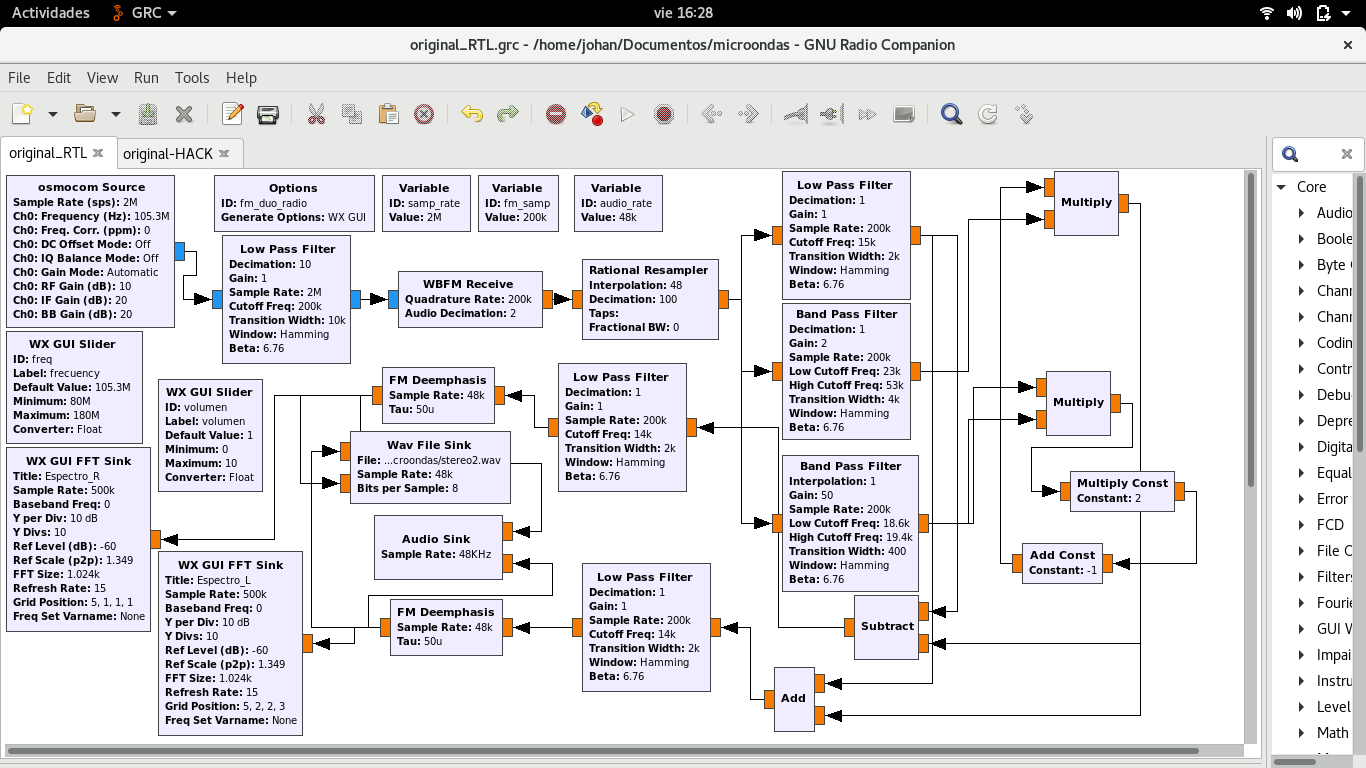
\includegraphics[width=\textwidth]{parte3/lab9/pdf/lab9_1.pdf}
\end{figure}

\end{frame}
%---------------------------------

\begin{frame}{Receptor FM Estereo}

\begin{itemize}
    \item {La FM, vino a cambiar en todo el esquema que existía en lo que a transmisión y recepción de radio se refiere.}
    \item {Una de las ventajas de FM estéreo es que la reproducción del sonido es tan buena en los receptores estereofónicos como en los de FM normal, estos lo reproducen como una señal monofónica de FM.}
\end{itemize}

\end{frame}
%---------------------------------

\begin{frame}{Receptor FM Estereo}

\begin{figure}[H]
\centering
\vspace{-3mm}
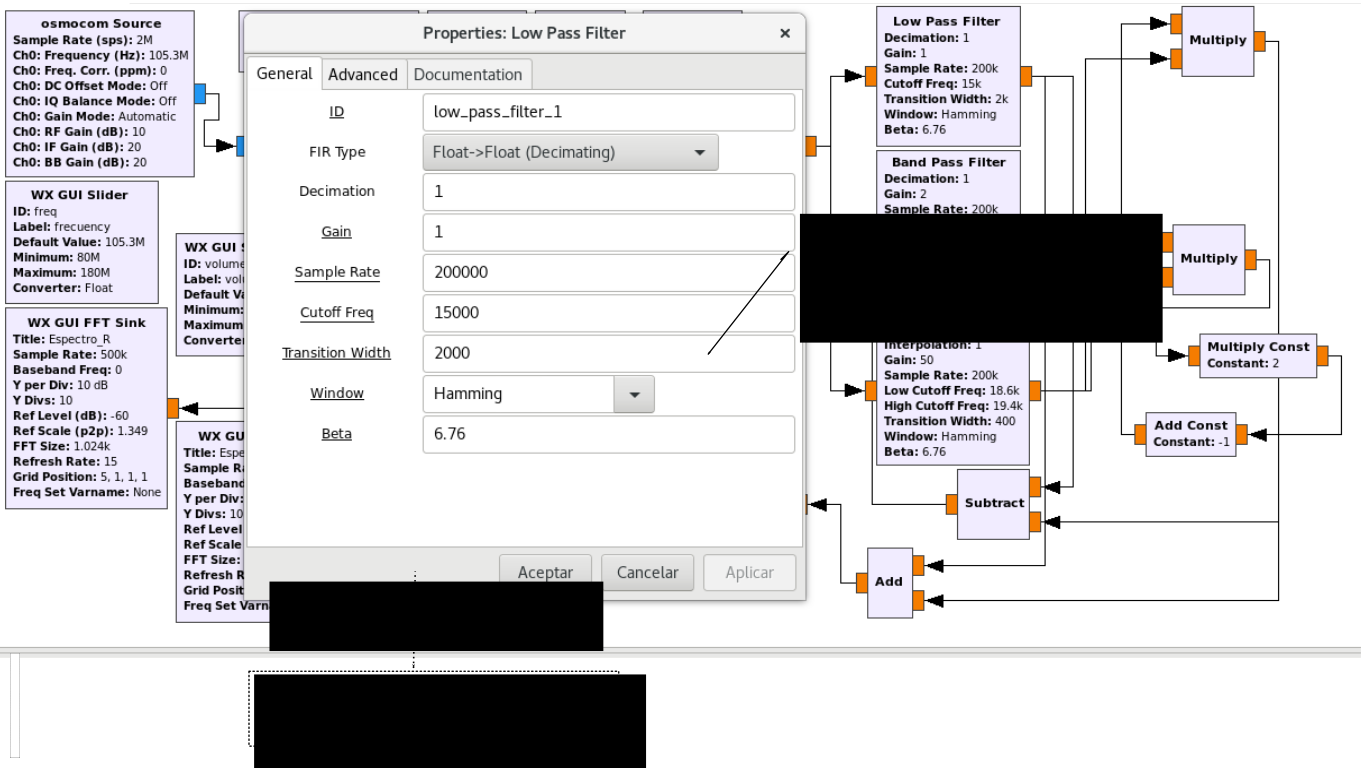
\includegraphics[width=\textwidth]{parte3/lab9/pdf/lab9_2.pdf}
\end{figure}

\end{frame}
%---------------------------------

\begin{frame}{Receptor FM Estereo}

\begin{figure}[H]
\centering
\vspace{-3mm}
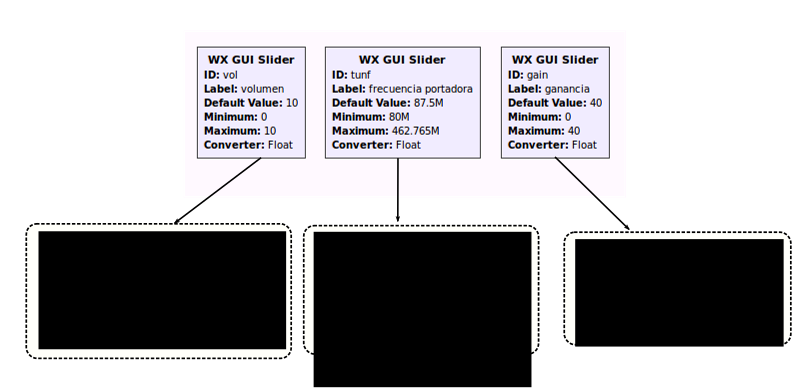
\includegraphics[width=\textwidth]{parte3/lab9/pdf/lab9_3.pdf}
\end{figure}

\end{frame}
%---------------------------------

\begin{frame}{Receptor FM Estereo}

\begin{figure}[H]
\centering
\vspace{-3mm}
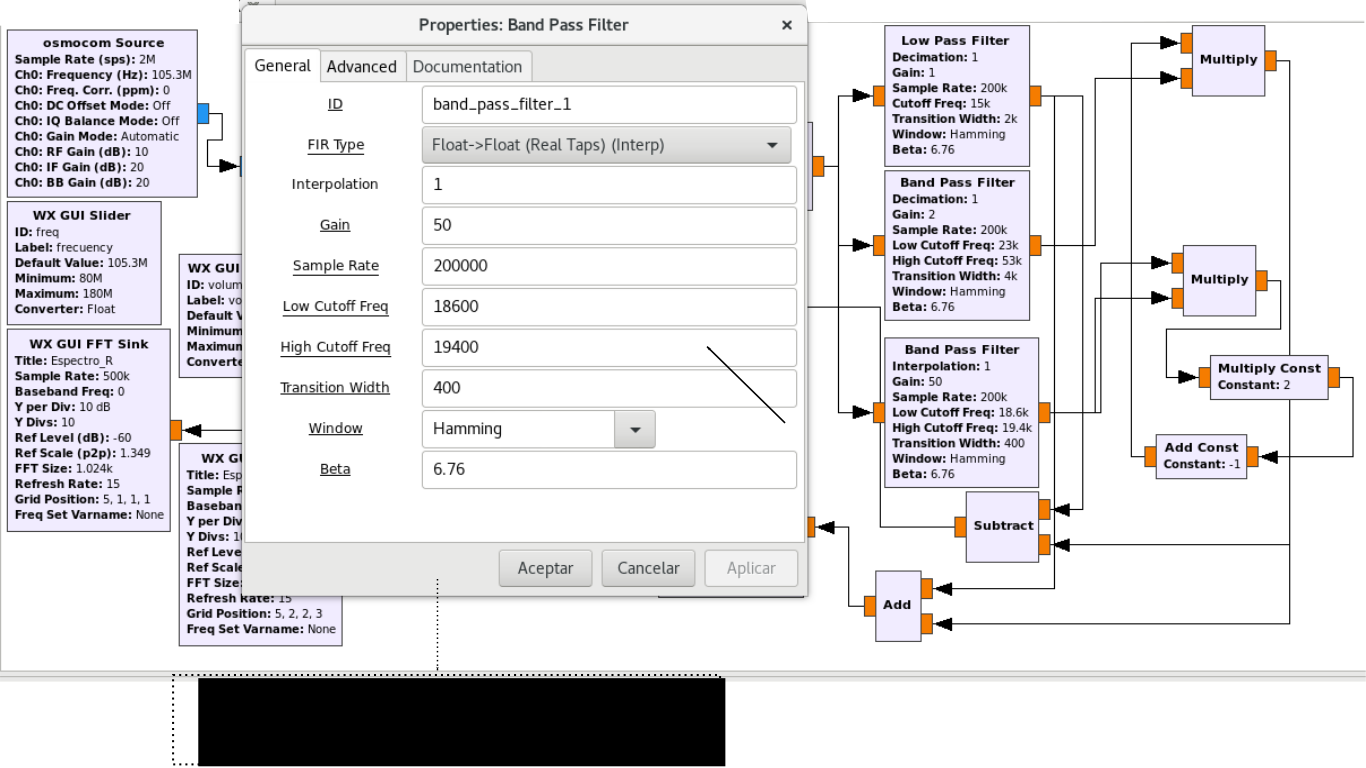
\includegraphics[width=\textwidth]{parte3/lab9/pdf/lab9_4.pdf}
\end{figure}

\end{frame}
%---------------------------------

\begin{frame}{Receptor FM Estereo}

\begin{figure}[H]
\centering
\vspace{-3mm}
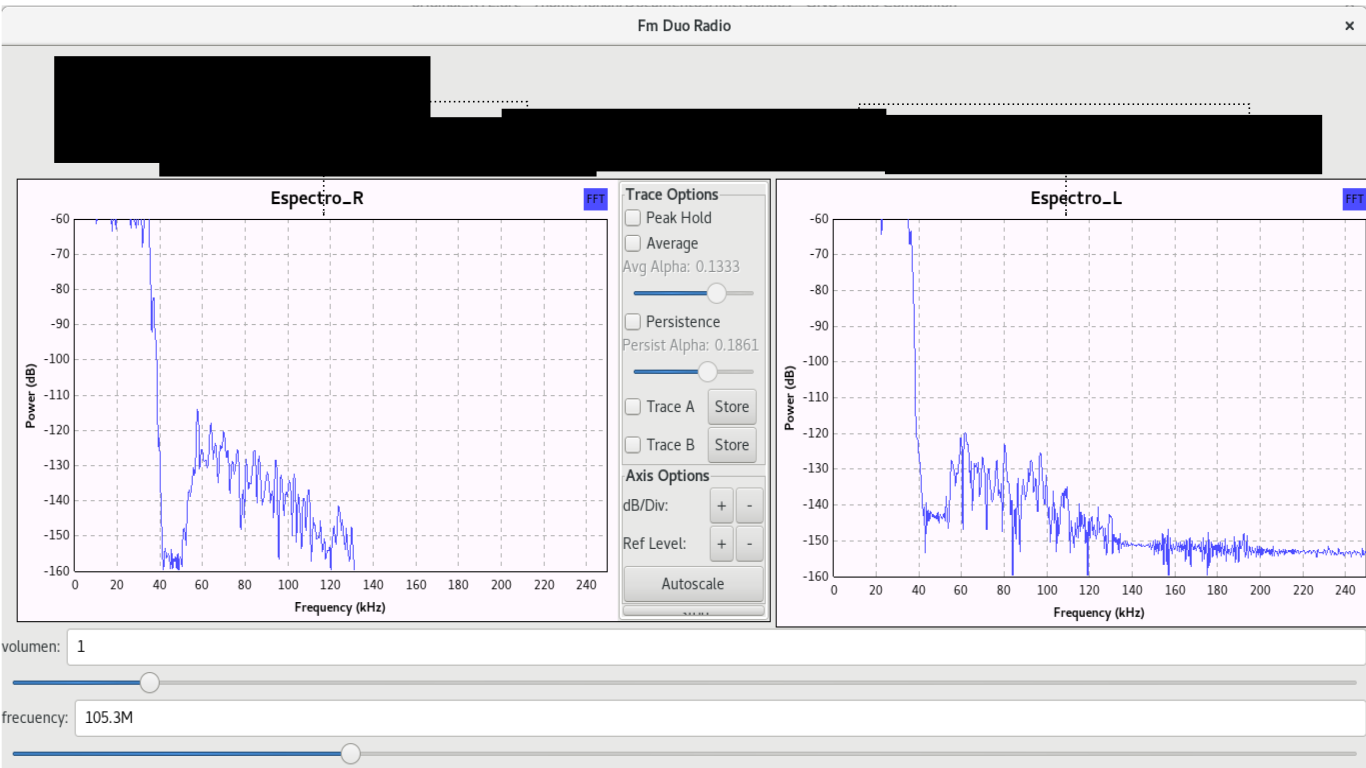
\includegraphics[width=\textwidth]{parte3/lab9/pdf/lab9_5.pdf}
\end{figure}

\end{frame}
%---------------------------------


%///////////////////////////////////////////////////////////////

\subsection{Lab11: Transmisor FM estereofónicofónico}

%*********************
\begin{frame}{}

\pgfdeclareimage[width=\paperwidth,height=\paperheight]{bg}{imagenes/fondo_lab}
\setbeamertemplate{background}{\pgfuseimage{bg}}

\bfseries{\textrm{\LARGE Lab11\\ \Large Transmisor FM estereofónico}}
\raggedright
\end{frame}
%*********************


\begin{frame}{Transmisor FM estereofónica}

\pgfdeclareimage[width=\paperwidth,height=\paperheight]{bg}{imagenes/fondo3}
\setbeamertemplate{background}{\pgfuseimage{bg}}

La transmisión FM estéreo es la emisión en frecuencia modulada por dos canales. Para emitir en estéreo no se emite directamente la señal R (Right o Derecha) y la señal L (Left o Izquierda) sino que se emiten las señales L-R por un canal y L+R por el otro. Esto se realiza con el fin de dar cualidades y calidades de sonido estéreo a la transmisión por frecuencia modulada.

\end{frame}
%---------------------------------

\begin{frame}{Transmisor FM estereofónico}
    
\begin{figure}[H]
\centering
\vspace{-3mm}
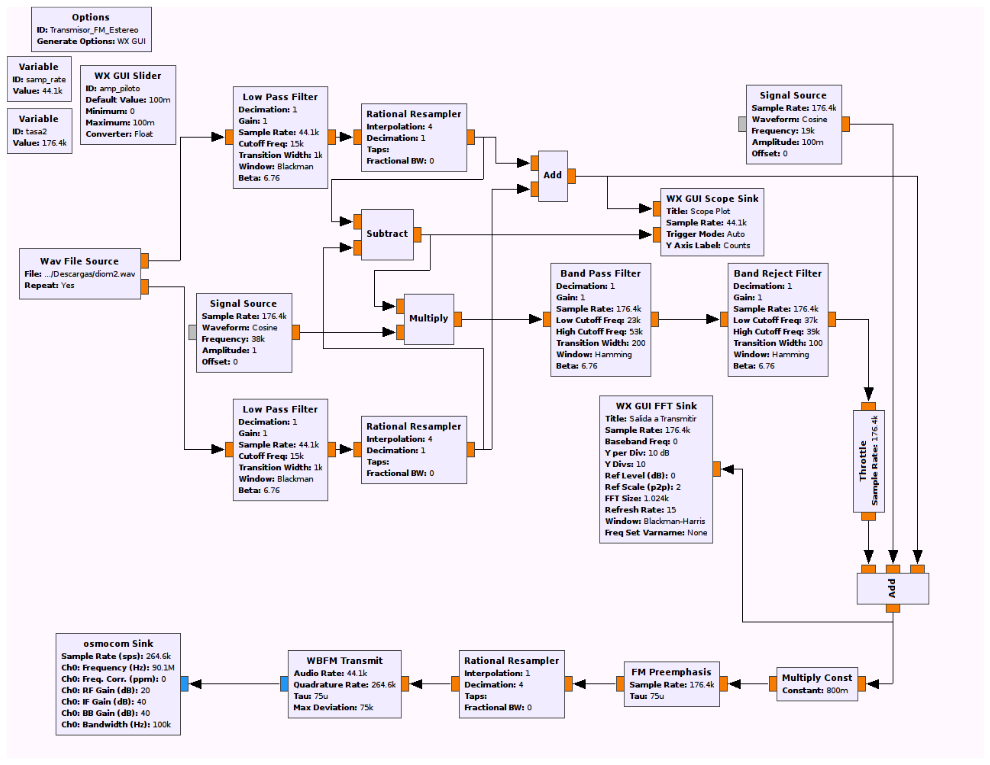
\includegraphics[width=.8\textwidth]{parte3/lab12/pdf/lab12_1.pdf}
\end{figure}
    
\end{frame}
%---------------------------------

\begin{frame}{Transmisor FM estereofónico}

\begin{figure}[H]
\centering
\vspace{-3mm}
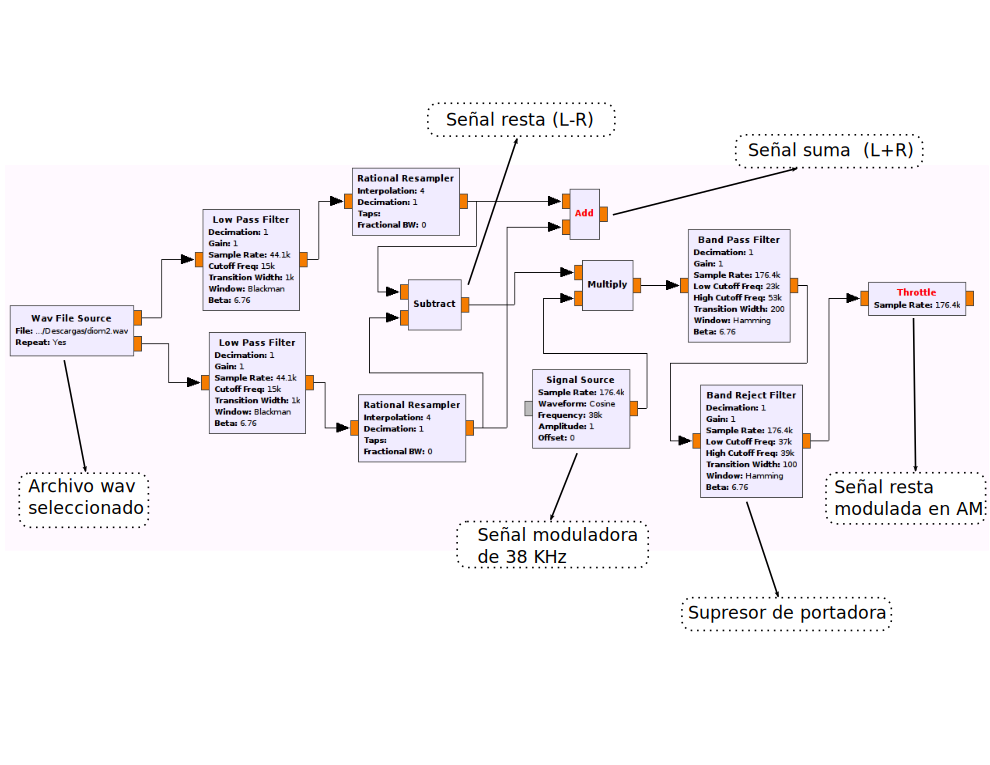
\includegraphics[width=\textwidth]{parte3/lab12/pdf/lab12_2.pdf}
\end{figure}
    
\end{frame}
%---------------------------------

\begin{frame}{Transmisor FM estereofónico}

\begin{figure}[H]
\centering
\vspace{-3mm}
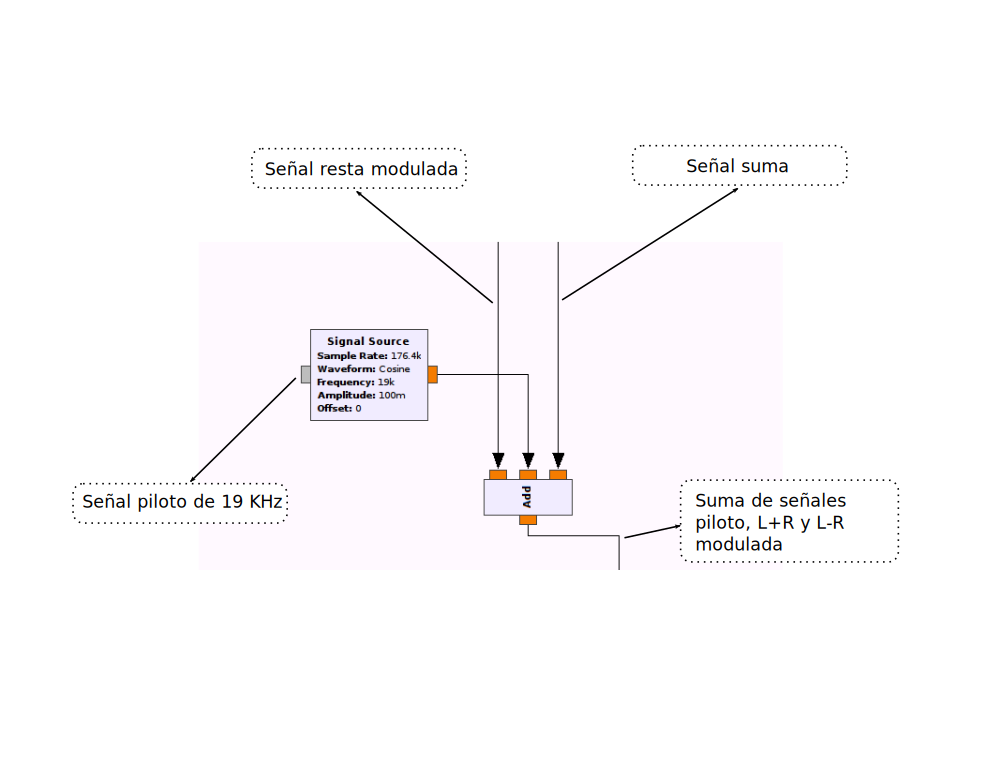
\includegraphics[width=\textwidth]{parte3/lab12/pdf/lab12_3.pdf}
\end{figure}
    
\end{frame}
%---------------------------------

\begin{frame}{Señal piloto de 19 KHz}

 El piloto estéreo es un tono de 19kHz que tiene la misma fase que la portadora de la Señal Resta (que hemos eliminado previamente), y una amplitud de (normalmente) el 10\% de la amplitud total de la señal, en caso de no detectarse el piloto es conveniente aumentar la amplitud del mismo hasta ser detectada por el receptor.
El piloto estéreo tiene tres funciones principales:

\begin{itemize}
    \item {Informa al receptor de que la emisión es estéreo}
    \item{Permite regenerar la subportadora de la Señal Resta a 38kHz que no hemos emitido gracias a modular en DSBSC.}
    \item{Permite regenerar la subportadora del RDS a 57kHz que no hemos emitido gracias a modular en DSBSC.}
\end{itemize}
    
\end{frame}
%---------------------------------

\begin{frame}{Transmisor FM estereofónico}

\begin{figure}[H]
\centering
\vspace{-3mm}
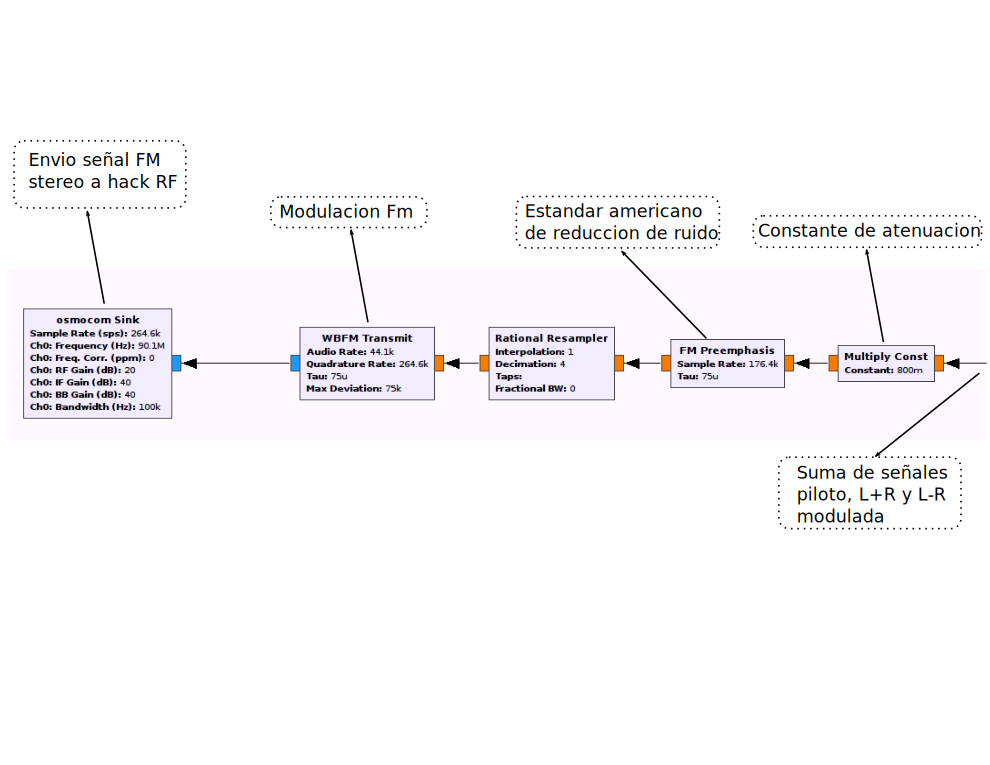
\includegraphics[width=\textwidth]{parte3/lab12/pdf/lab12_4.pdf}
\end{figure}
    
\end{frame}
%---------------------------------

\begin{frame}{Transmisor FM estereofónico}

\begin{figure}[H]
\centering
\vspace{-3mm}
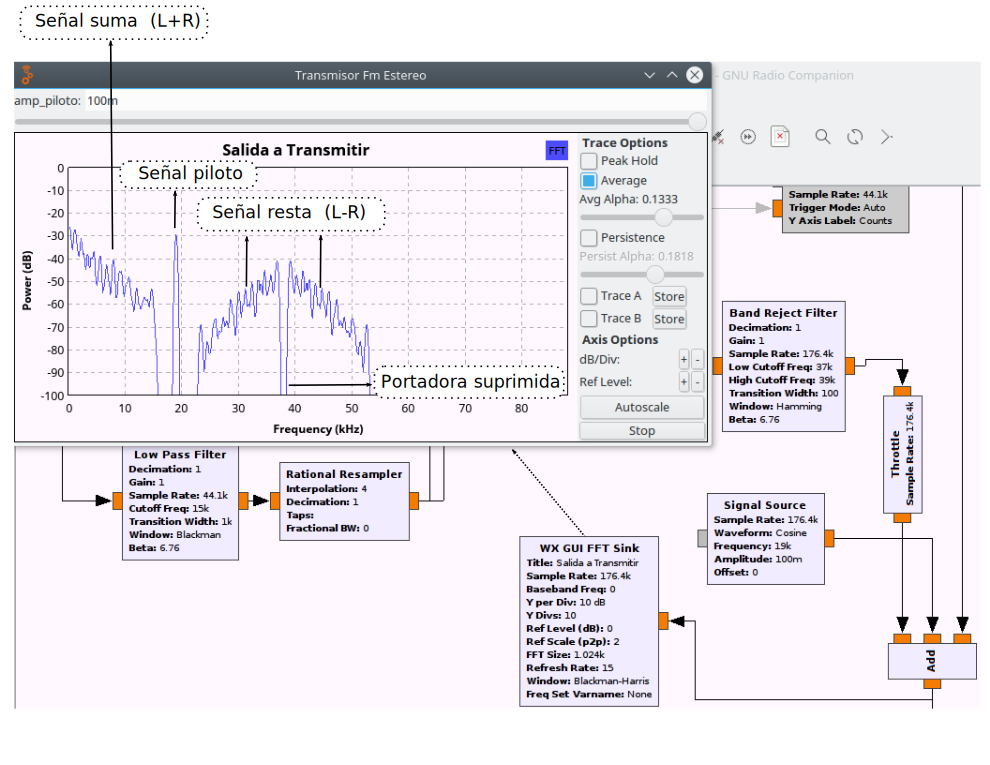
\includegraphics[width=.9\textwidth]{parte3/lab12/pdf/lab12_5.pdf}
\end{figure}
    
\end{frame}
%---------------------------------

%///////////////////////////////////////////////////////////////

\subsection{Lab13: Transmisor FM Estereo FIFO}

%*********************
\begin{frame}{}

\pgfdeclareimage[width=\paperwidth,height=\paperheight]{bg}{imagenes/fondo_lab}
\setbeamertemplate{background}{\pgfuseimage{bg}}

\bfseries{\textrm{\LARGE Lab13\\ \Large Transmisor FM Estereo FIFO}}
\raggedright
\end{frame}
%*********************

\begin{frame}{Introducción}

\pgfdeclareimage[width=\paperwidth,height=\paperheight]{bg}{imagenes/fondo3}
\setbeamertemplate{background}{\pgfuseimage{bg}}

Se realizará la retransmisión de una emisora online utilizando el transmisor de FM estéreo construido previamente en GNU radio (practica anterior); se aprovechará  la característica de un archivo “conducto” o “tubería” el cual nos permite que procesos separados se comuniquen sin haber sido diseñados para funcionar juntos; gracias a la herramienta mpg123 es posible alimentar un archivo FIFO que se comporta como tubería; es decir en la medida que ingresan los bits de información de la emisora online en la “tubería”, así mismo son extraídos por el transmisor de radio FM estéreo.

\end{frame}
%---------------------------------

\begin{frame}{Esquema general}
    
\begin{figure}[H]
\centering
\vspace{-3mm}
\includegraphics[width=\textwidth]{parte3/lab13/pdf/lab13_1.pdf}
\end{figure}
    
\end{frame}
%---------------------------------

\begin{frame}{Obtención URL emisora online}
    
\begin{figure}[H]
\centering
\vspace{-3mm}
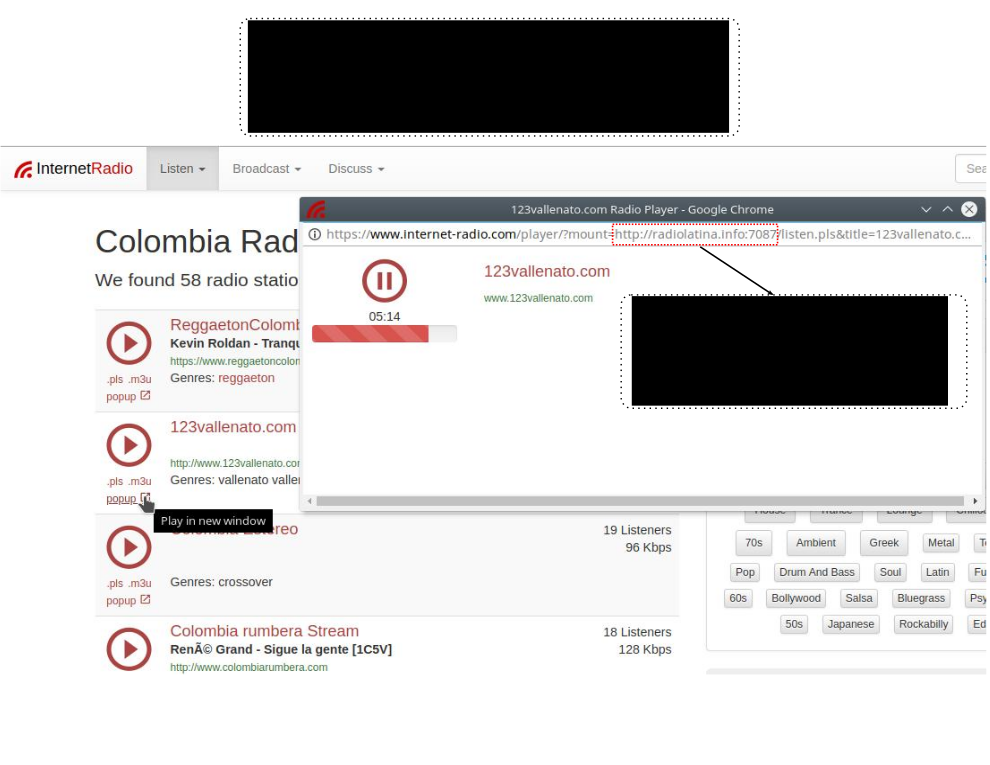
\includegraphics[width=.9\textwidth]{parte3/lab13/pdf/lab13_2.pdf}
\end{figure}
    
\end{frame}
%---------------------------------

\begin{frame}{Creación archivo FIFO}

Existe un tipo de tubería que puede ser descrita como una tubería "con nombre", también denominada FIFO que sus siglas traducen "Primero en entrar, primero en salir" y se refiere a la propiedad de que el orden de bytes entrante es el mismo que sale.

\begin{itemize}
    \item {Mediante el uso de consola procedemos a introducir el comando mkfifo, que nos permite crear el archivo FIFO.
    
    \begin{block}{}
    \texttt{
    \ \ \ mkfifo emisora\_online.fifo}
    \end{block}
    }
    \item {Mediante la herramienta mpg123 se procede a alimentar el archivo FIFO con una emisora online.
    
    \begin{block}{}
    \texttt{
    \ \ \ mpg123 -r44100 --stereo -s http://radiolatina.info:7087>emisora\_online.fifo}
    \end{block}
    }
\end{itemize}
\end{frame}
%---------------------------------

\begin{frame}{Creación archivo FIFO}

La opción "--stereo" permite realizar una transmisión de tipo estéreo, utilice “-m” para realizar una transmisión de tipo monofónica.\vspace{2mm}

Con la ayuda de la apción “-r” podemos definir la tasa de muestreo, por ejemplo "-r44100" convierte la frecuencia de muestreo a 44100 muestras por segundo. \vspace{2mm}

Es importante el uso del comando “-s” que nos permite que las muestras de audio decodificadas se escriben en la salida estándar es decir en consola, en lugar de reproducirlas a través del dispositivo de audio; gracias a esta característica se puede llevar a cabo el concepto del uso de tuberías que suelen ser alimentadas a través de pantalla.

\end{frame}
%---------------------------------

\begin{frame}{Creación archivo FIFO}

\begin{itemize}
    \item {Si se desea realizar una prueba previa a la transmisión, es posible escuchar la emisora de igual manera mediante la herramienta mpg123; recuerde eliminar el comando “-s” para que las muestras de audio no se muestren en pantalla y sean reproducidas a través del dispositivo de audio.
    
    \begin{block}{}
    \texttt{
    \ \ \ mpg123 -r44100 --stereo  http://radiolatina.info:7087}
    \end{block}
    }
\end{itemize}
\end{frame}
%---------------------------------

\begin{frame}{Explicación bloques extras}

\begin{figure}[H]
\centering
\vspace{-3mm}
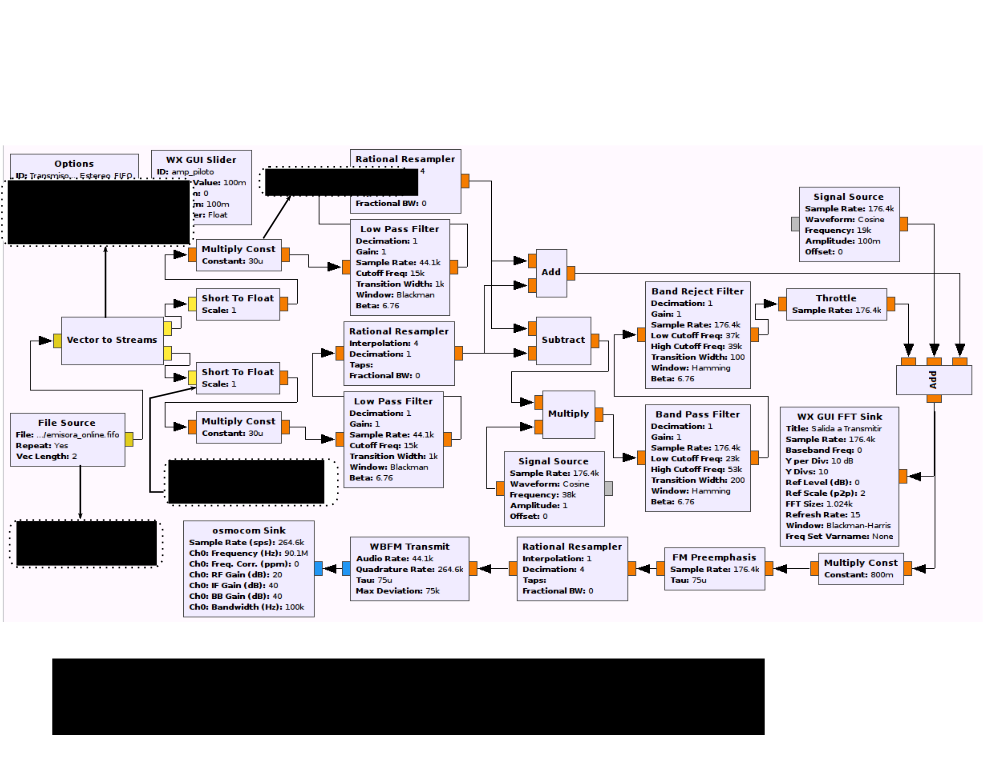
\includegraphics[width=\textwidth]{parte3/lab13/pdf/lab13_3.pdf}
\end{figure}
\end{frame}
%---------------------------------

\begin{frame}{Espectro de señal a transmitir}

\begin{figure}[H]
\centering
\vspace{-3mm}
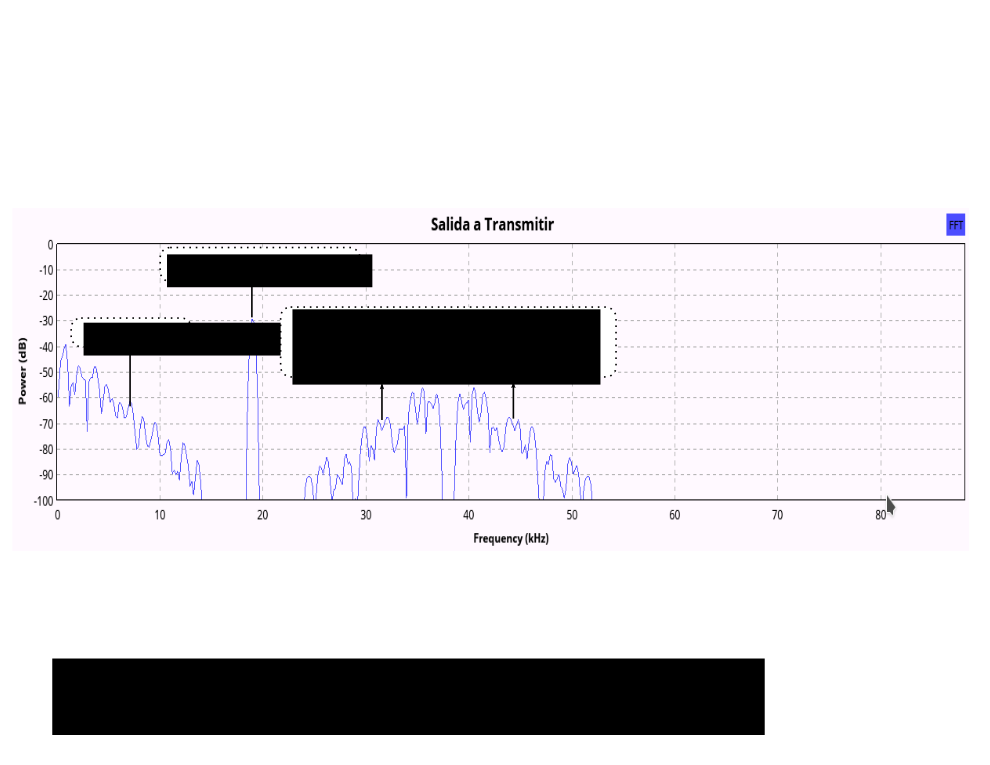
\includegraphics[width=\textwidth]{parte3/lab13/pdf/lab13_4.pdf}
\end{figure}
\end{frame}
%---------------------------------   %Cambiar nombre

%///////////////////////////////////////////////////////////////

\subsection{Lab10: Señales FM para Walkie-Talkie}
%*********************
\begin{frame}{}

\pgfdeclareimage[width=\paperwidth,height=\paperheight]{bg}{imagenes/fondo_lab}
\setbeamertemplate{background}{\pgfuseimage{bg}}


\bfseries{\textrm{\LARGE Lab10 \newline\Large Transmisión y recepción de \newline señales de radio FM para \newline Walkie-Talkie}}
\raggedright
\end{frame}
%*********************

\begin{frame}{Recepción de señales de radio FM para un Walkie-Talkie}

\pgfdeclareimage[width=\paperwidth,height=\paperheight]{bg}{imagenes/fondo3}
\setbeamertemplate{background}{\pgfuseimage{bg}}

Para esta práctica se realiza el diagrama de bloques en el software GNU-Radio, esto se hace para captar las señales de las frecuencias portadoras de cada uno de los canales del radio EP150, a continuación se muestra el radio utilizado en esta práctica y su respectiva tabla de especificaciones, estas son necesarias durante la práctica, también se presenta el diagrama de bloques realizado para la captación de las portadoras.
    
\end{frame}
%---------------------------------

\begin{frame}{EP150}

El EP150 presenta facilidad de uso, mantiene sus operaciones según lo programado, maximiza la productividad de los turnos laborales, mejorar la  seguridad y aumentar la satisfacción general de los clientes. El versátil EP150 es compatible con otros radios que funcionen en la misma frecuencia y código, y también tiene un complemento de accesorios para hacer que el radio se ajuste a sus necesidades.

\begin{figure}[H]
\centering
\vspace{-3mm}
\includegraphics[width=.3\textwidth]{parte3/lab10/pdf/lab10_1.pdf}
\end{figure}

\centering\tiny{Modelo EP150 UHF}

\end{frame}
%---------------------------------

\begin{frame}{Especificaciones del radio}

Estas especificaciones serán necesarias con el fin de conocer el rango de frecuencia de operación del radio.

\begin{figure}[H]
\centering
\vspace{-3mm}
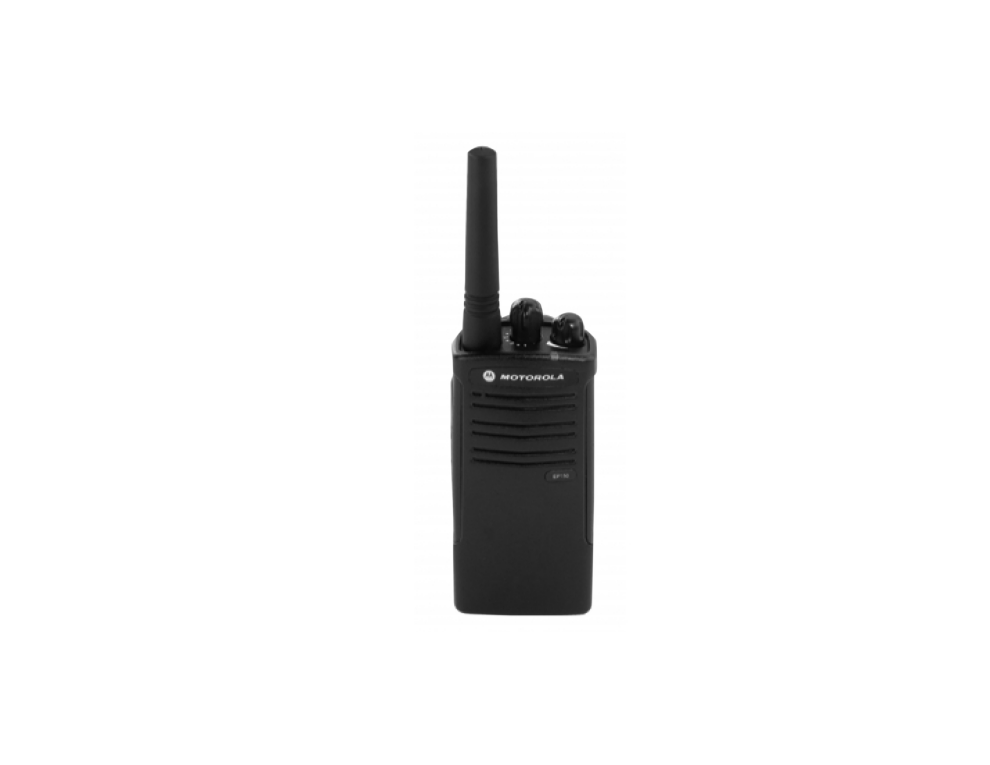
\includegraphics[width=\textwidth]{parte3/lab10/pdf/lab10_2.pdf}
\end{figure}

\end{frame}
%---------------------------------

\begin{frame}{GQRX}

Es necesario instalar el programa gqrx, útil para determinar las frecuencias de trabajo del radio en cada uno de sus canales, para instalarlo se usa:

\begin{block}{}
  \texttt{
  \ \ \ sudo apt-get update
    \begin{itemize}
      \item[] sudo apt-get install gqrx-sdr
    \end{itemize}}
\end{block}

\end{frame}
%---------------------------------

\begin{frame}{HackRF One}

Al iniciar el programa se configura el dispositivo, en este caso una Hack RF. Para verificar que este conectada al PC se puede usar la órden:

\begin{block}{}
  \texttt{
  \ \ \ hackrf\_info}
\end{block}

\begin{figure}[H]
\centering
\vspace{-3mm}
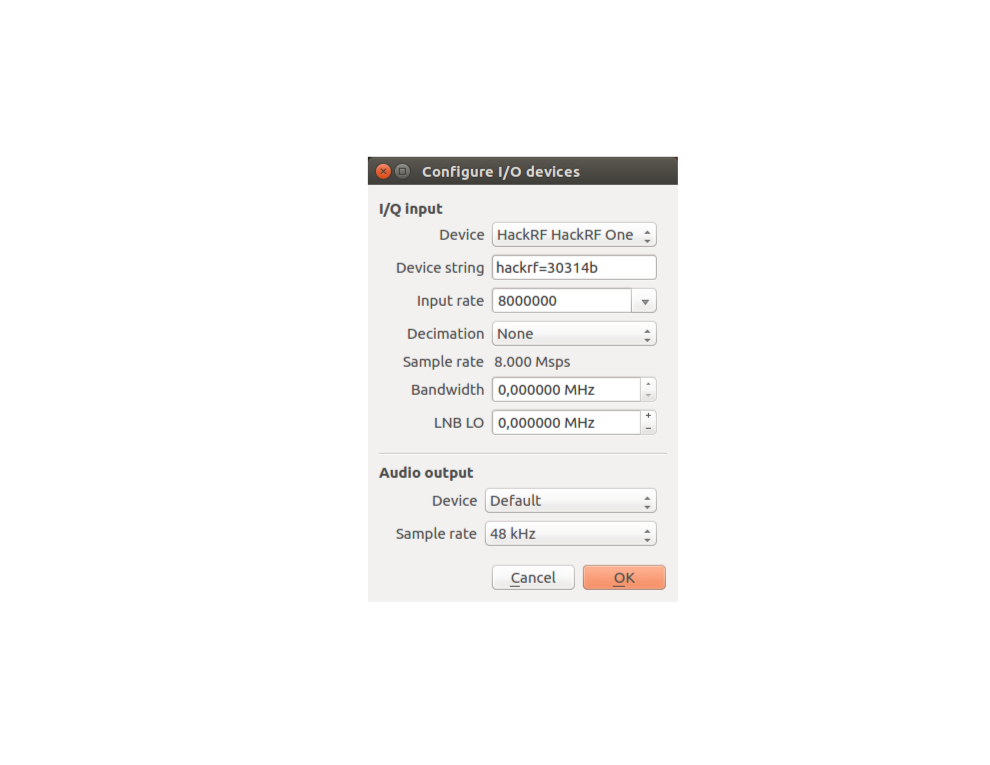
\includegraphics[width=.3\textwidth]{parte3/lab10/pdf/lab10_3.pdf}
\end{figure}

\end{frame}
%---------------------------------

\begin{frame}{Interfaz del programa}

\begin{figure}[H]
\centering
\vspace{-3mm}
\includegraphics[width=.9\textwidth]{parte3/lab10/pdf/lab10_4.pdf}
\end{figure}

\end{frame}
%---------------------------------

\begin{frame}{Detectar frecuencias}

\begin{figure}[H]
\centering
\vspace{-3mm}
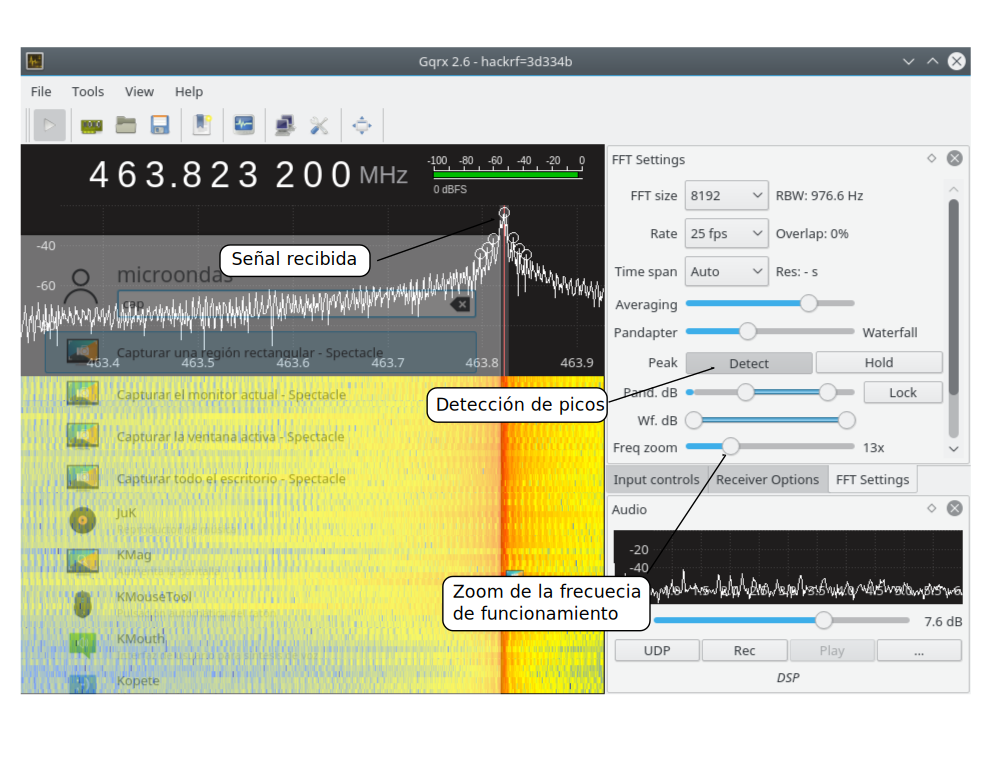
\includegraphics[width=\textwidth]{parte3/lab10/pdf/lab10_5.pdf}
\end{figure}

\end{frame}
%---------------------------------

\begin{frame}{Tabla de frecuencias}

Al variar los 8 canales disponibles del dispositivo, se logran encontrar las frecuencias correspondientes.

\begin{figure}[H]
\centering
\vspace{-3mm}
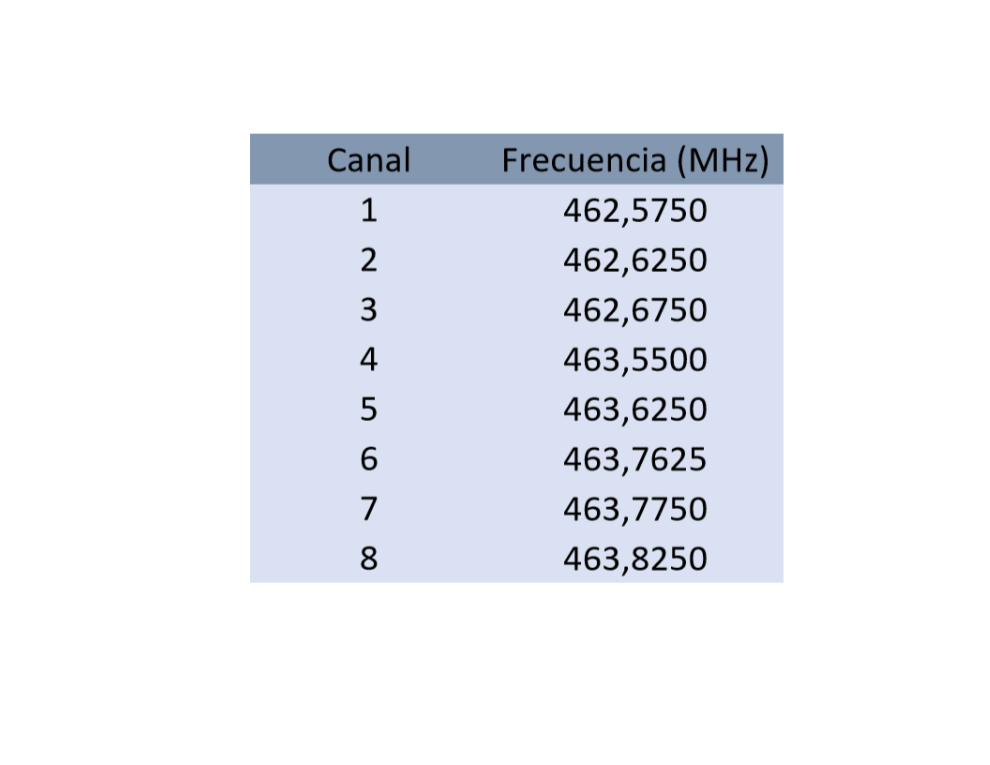
\includegraphics[width=.8\textwidth]{parte3/lab10/pdf/lab10_6.pdf}
\end{figure}

\end{frame}
%---------------------------------

\begin{frame}{}

Obtenidos los rangos de frecuencias de cada uno de los canales del radio, se realiza el diagrama de bloques en GNU Radio con el fin de observar las señales portadoras de cada uno de los canales en un osciloscopio.

\begin{figure}[H]
\centering
\vspace{-3mm}
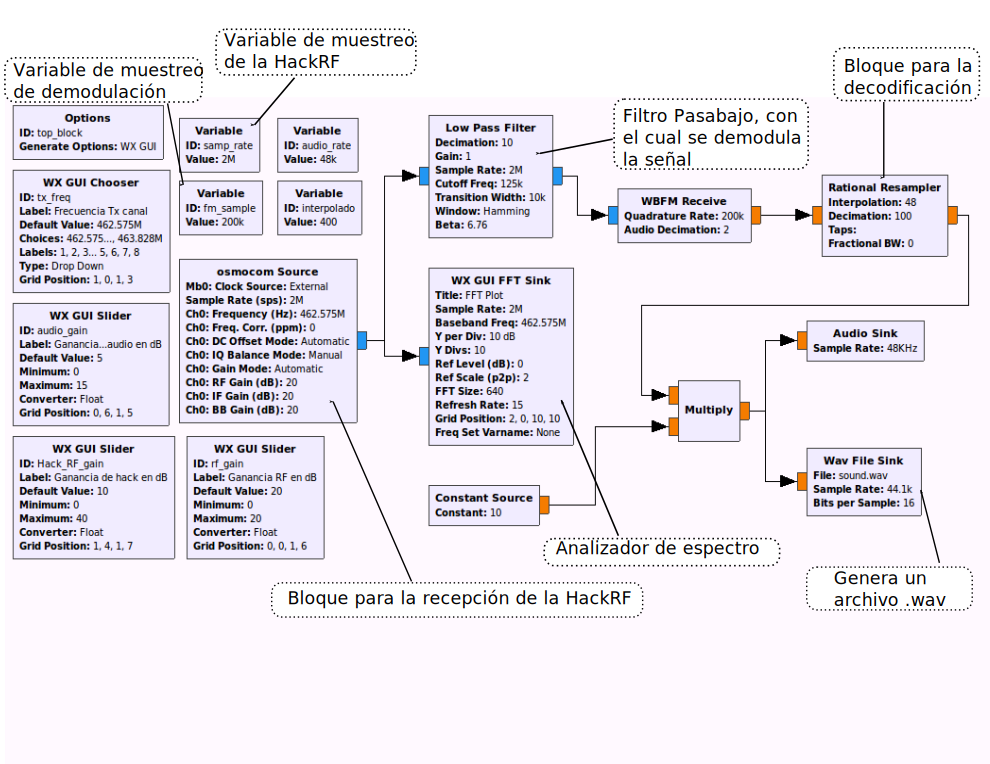
\includegraphics[width=.9\textwidth]{parte3/lab10/pdf/lab10_7.pdf}
\end{figure}

\end{frame}
%---------------------------------

\begin{frame}{Configuraciones}

Se configura el bloque con el que se recepciona la señal con la tarjeta HackRF donde nos permite configurar mas de una tarjeta en la misma conexión.

\begin{figure}[H]
\centering
\vspace{-3mm}
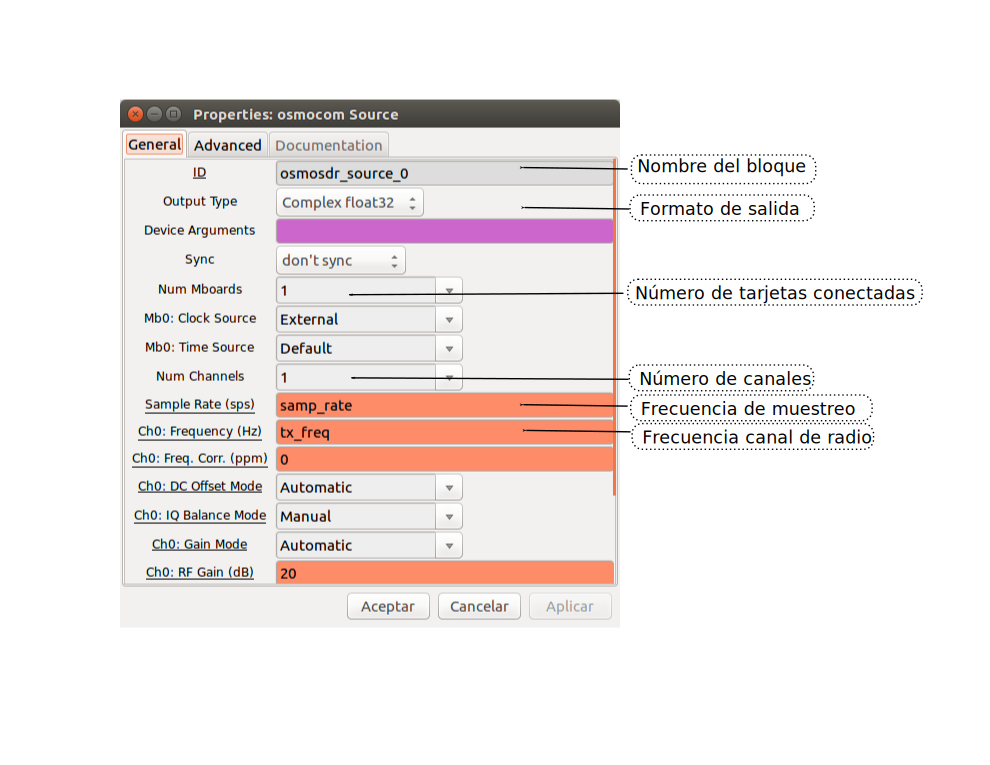
\includegraphics[width=.8\textwidth]{parte3/lab10/pdf/lab10_8.pdf}
\end{figure}

\end{frame}
%---------------------------------

\begin{frame}{Configuraciones}

Se configura el bloque con el que se demodula la señal con la tarjeta HackRF.

\begin{figure}[H]
\centering
\vspace{-3mm}
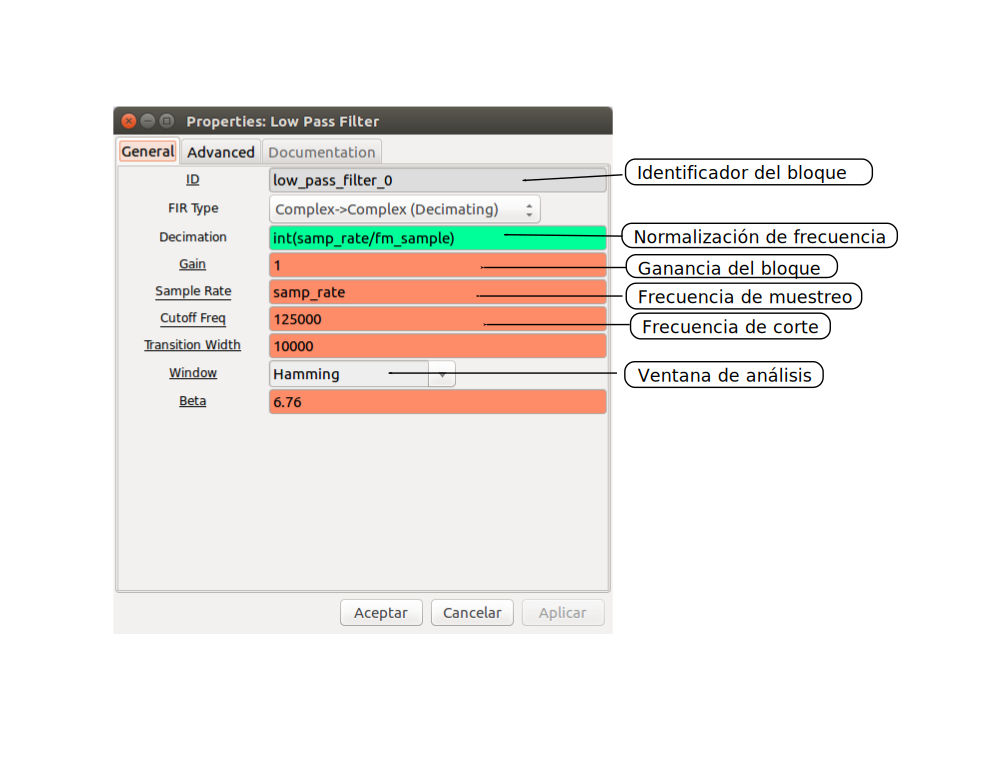
\includegraphics[width=.8\textwidth]{parte3/lab10/pdf/lab10_9.pdf}
\end{figure}

\end{frame}
%---------------------------------

\begin{frame}{Configuraciones}

Se configura el bloque con el cual se decodifica la información mediante una comparación de frecuencias:

\begin{figure}[H]
\centering
\vspace{-3mm}
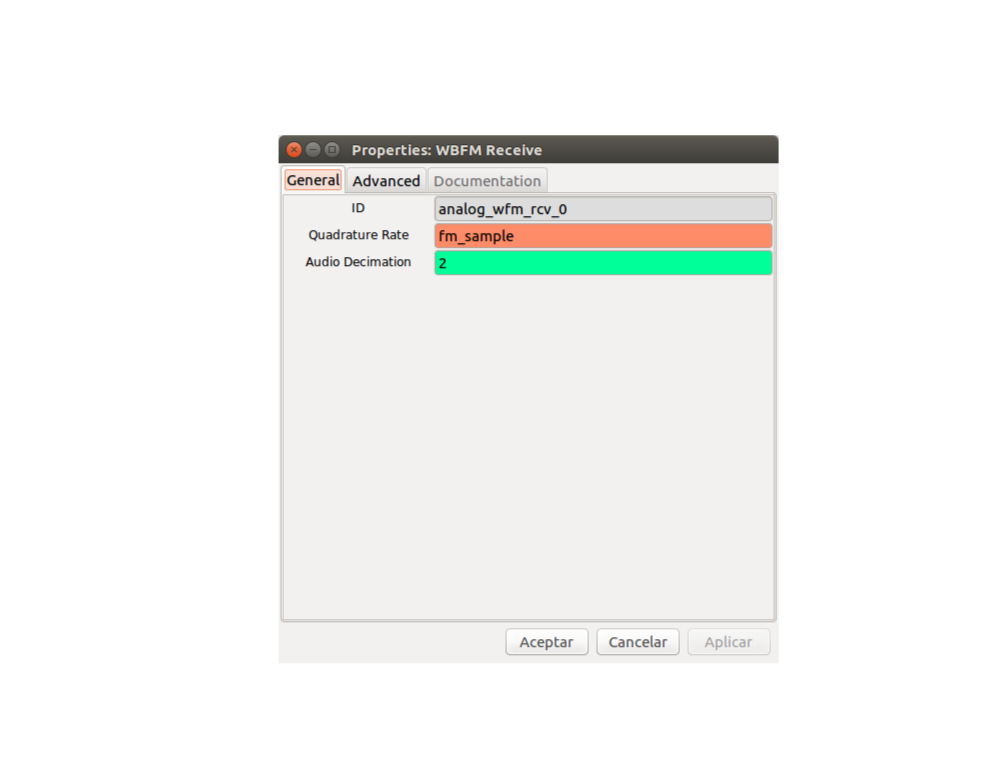
\includegraphics[width=.5\textwidth]{parte3/lab10/pdf/lab10_10.pdf}
\end{figure}

\end{frame}
%---------------------------------

\begin{frame}{Configuraciones}

Se configura el bloque que se utiliza como el selector de canal:

\begin{figure}[H]
\centering
\vspace{-3mm}
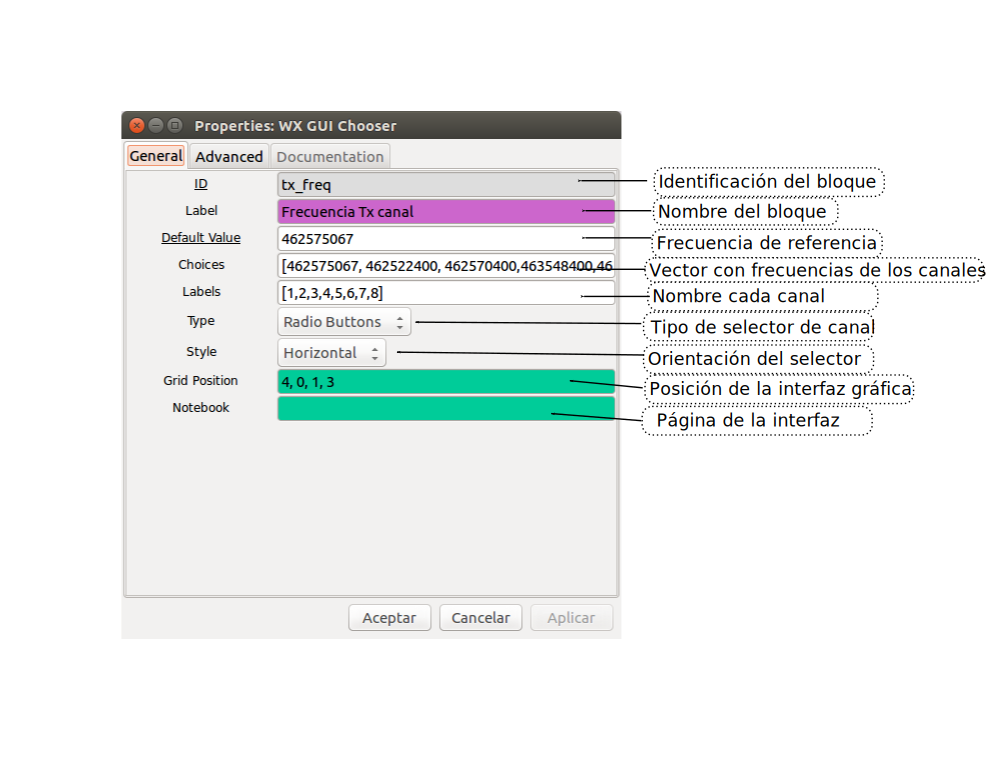
\includegraphics[width=\textwidth]{parte3/lab10/pdf/lab10_11.pdf}
\end{figure}

\end{frame}
%---------------------------------

\begin{frame}{Interfaz gráfica para la demodulación de la señal}

\begin{figure}[H]
\centering
\vspace{-3mm}
\includegraphics[width=\textwidth]{parte3/lab10/pdf/lab10_12.pdf}
\end{figure}

\end{frame}
%---------------------------------

\begin{frame}{Conclusión}

Se observa y escucha la señal recibida por el EP150 y eventualmente la señal que envía una Hack RF transmisora de FM. El tiempo que corre el programa y esta la interfaz abierta graba y deposita la información en un WAV.

\end{frame}
%---------------------------------

   %Cambiar nombre - es solo transmisión o recepción

%///////////////////////////////////////////////////////////////

\subsection{Lab14: Tx FM para Walkie-Talkie UHF}

%*********************
\begin{frame}{}

\pgfdeclareimage[width=\paperwidth,height=\paperheight]{bg}{imagenes/fondo_lab}
\setbeamertemplate{background}{\pgfuseimage{bg}}

\bfseries{\textrm{\LARGE Lab14 \newline \Large Transmisión de señales FM \newline para radio Walkie-Talkie en la \newline banda UHF por medio de SDR
}}
\raggedright
\end{frame}
%*********************


\begin{frame}{Transmisión FM para Walkie-Talkie UHF}

\pgfdeclareimage[width=\paperwidth,height=\paperheight]{bg}{imagenes/fondo3}
\setbeamertemplate{background}{\pgfuseimage{bg}}

Para este laboratorio se construirá un diagrama de bloques utilizando el software GNU Radio que nos permitirá realizar prácticas a través de radio definido por software, con el fin de realizar la transmisión de las señales de radiofrecuencia modulada en la banda de UHF en donde se encuentran las frecuencias de cada uno de los canales del dispositivo Motorola EP150, el cual será utilizado para llevar acabo correctamente la práctica.
\end{frame}
%---------------------------------

\begin{frame}{Tonos privados}

\textbf{CTCSS}\\
\vspace{3mm}
El sistema continuo de silenciamiento codificado por tonos o CTCSS es un circuito que se utiliza para reducir la molestia de escuchar a otros usuarios en un canal compartido de comunicaciones de radio bidireccionales. A veces se lo conoce como silenciamiento de tono. Lo hace agregando un tono de audio de baja frecuencia a la voz. Cuando más de un grupo de usuarios está en la misma frecuencia de radio (llamados usuarios co-canal), los circuitos CTCSS silencian a los usuarios que están utilizando un tono CTCSS diferente o no CTCSS. (Wikipedia, 2018).
\end{frame}
%---------------------------------

\begin{frame}{Detección de portadoras y tonos privados}

Para este procedimiento es necesario contar con el software SDR-Sharp el cual es un analizador de espectro de frecuencias y además cuenta con la función de detector de tonos privados CTCSS (actualmente solo cuenta con soporte para Windows), sumado a esto también se utilizará el dispositivo HackRF-One como receptor de señales FM, además del transmisor Motorola EP150. (Airspy, 2018).

\end{frame}
%---------------------------------

\begin{frame}{Detección de portadoras y tonos privados}

\begin{figure}[H]
\centering
\vspace{-3mm}
\includegraphics[width=0.9\textwidth]{parte3/lab14/pdf/Lab14_1.pdf}
\end{figure}

\end{frame}
%---------------------------------

\begin{frame}{Frecuencias de la señal de portadora}

Como se mostró en la figura anterior se pueden observar la frecuencia de las portadoras de cada canal y su respectivo tono CTCSS el cual es de 67Hz como se muestra en la siguiente tabla, dado el caso de que las portadoras halladas y sus tonos no correspondan con la tabla es necesario reiniciar el dispositivo a sus valores de fabrica véase el manual. (Motorola, 2010) 


\begin{table}[]
\scriptsize
\centering
\begin{tabular}{|c|c|}
\hline

\rowcolor{BlueGreen!20}
\textbf{CANAL} & \textbf{FRECUENCIA DE SEÑAL PORTADORA} \\ \hline
1              & 462,5750 MHz                           \\ \hline
2              & 462,6250 MHz                           \\ \hline
3              & 462,6750 MHz                           \\ \hline
4              & 463,5500 MHz                           \\ \hline
5              & 463,6250 MHz                           \\ \hline
6              & 463,7625 MHz                           \\ \hline
7              & 463,7750 MHz                           \\ \hline
8              & 463,8250 MHz                           \\ \hline
\end{tabular}
\end{table}

\end{frame}
%---------------------------------

\begin{frame}{Desarrollo del diagrama en GNU Radio}
Para la transmisión de la señal FM para el Walkie-Talkie se desarrolló el siguiente esquema:

\begin{figure}[H]
\centering
\vspace{-1mm}
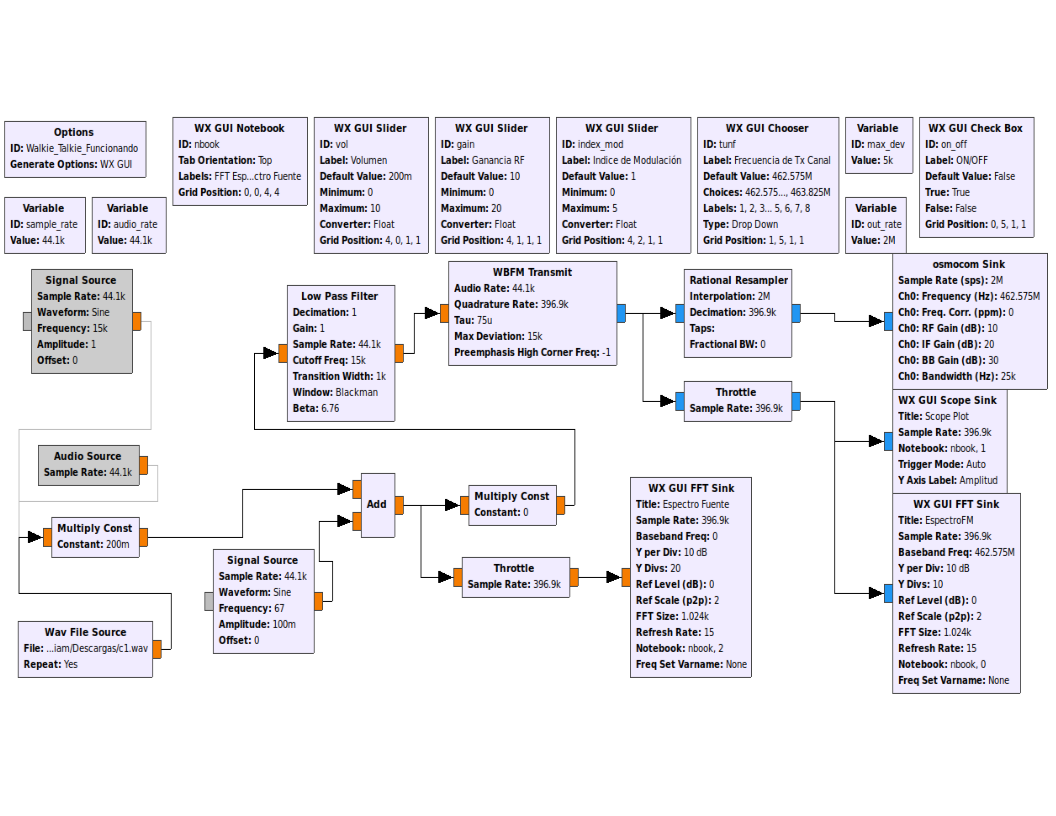
\includegraphics[width=\textwidth]{parte3/lab14/pdf/Lab14_2.pdf}
\end{figure}

\end{frame}
%---------------------------------

\begin{frame}{Desarrollo del diagrama en GNU Radio}

Las variables necesarias para el desarrollo del esquema son:
\begin{itemize}
    \item {\textit{sample\_rate} = Frecuencia de muestreo general}
    \item {\textit{audio\_rate} = Frecuencia de muestreo del audio (se suele utilizar 44.1KHz)}
    \item {\textit{out\_rate} = Frecuencia de muestreo del dispositivo HackRF-One}
    \item {\textit{max\_dev} = Desviación máxima en frecuencia de la señal modulada (viene dada por el producto index\_mod*15KHz el cual es el estándar para WBFM)}
    
\end{itemize}{}

\end{frame}
%---------------------------------

\begin{frame}{Desarrollo del diagrama en GNU Radio}

También es necesario utilizar un grupo de slider entre los que encontramos:
\begin{itemize}
    \item {\textit{vol}  = Volumen del audio}
    \item {\textit{index\_mod} = Índice de modulación (suele utilizarse un índice entre 1 y 5)}
    \item {\textit{gain} = Ganancia RF (ganancia prevista por parte de la tarjeta)}
    \item {\textit{tunf} = Frecuencia de Tx (frecuencia de las distintas portadoras de los canales)}
    
\end{itemize}{}

\end{frame}
%---------------------------------

\begin{frame}{Desarrollo del diagrama en GNU Radio}

Para comenzar con el diagrama de transmisiones es necesario incluir el audio que se desea transmitir esto se puede lograr cargando un archivo WAV (bloque WAV file source), mediante el micrófono del equipo (bloque Audio Source) o finalmente a partir de un generador de señales (bloque Signal Source) seguido a esto se multiplica por una constante, cuyo valor esta dado por el slider vol, con el fin de obtener la amplitud deseada, dicha amplitud no debe exceder los 200m, como se observa a continuación:

\begin{figure}[H]
\centering
\vspace{-3mm}
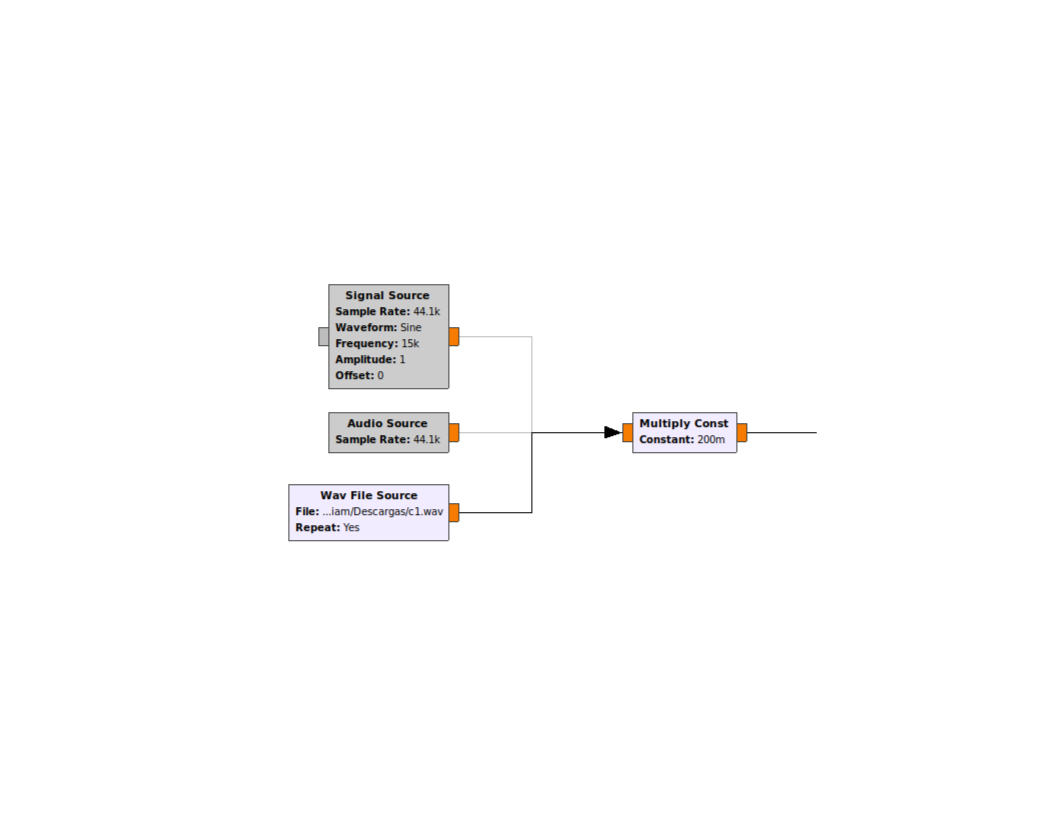
\includegraphics[width=0.7\textwidth]{parte3/lab14/pdf/Lab14_3.pdf}
\end{figure}


\end{frame}
%---------------------------------

\begin{frame}{Desarrollo del diagrama en GNU Radio}

Luego se añade el tono CTCSS a la información a transmitir esto con el fin de que la señal transmitida pueda ser escuchada desde el dispositivo Walkie-Talkie como se puede observar:

\begin{figure}[H]
\centering
\vspace{-3mm}
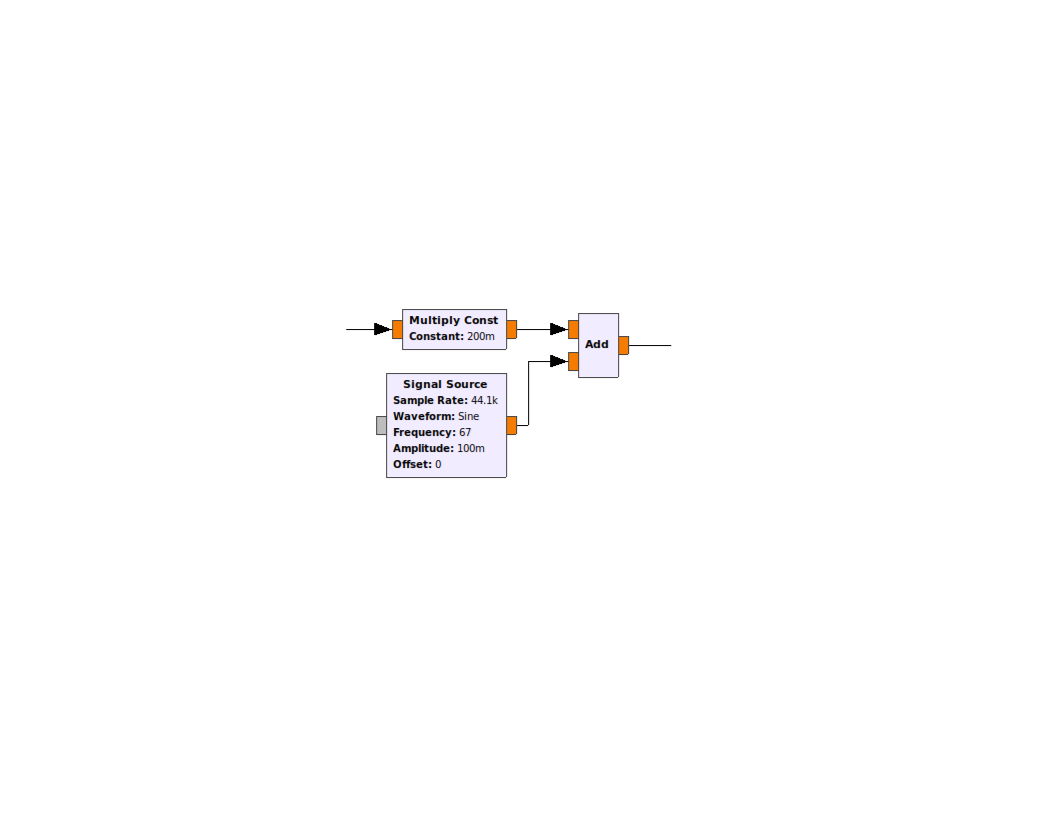
\includegraphics[width=0.6\textwidth]{parte3/lab14/pdf/Lab14_4.pdf}
\end{figure}

\end{frame}
%---------------------------------

\begin{frame}{Desarrollo del diagrama en GNU Radio}

En la siguiente etapa se implementa un filtro pasa bajas a la señal evitando frecuencias altas que pudieran llegar a contener ruido en la transmisión.

\begin{figure}[H]
\centering
\vspace{-3mm}
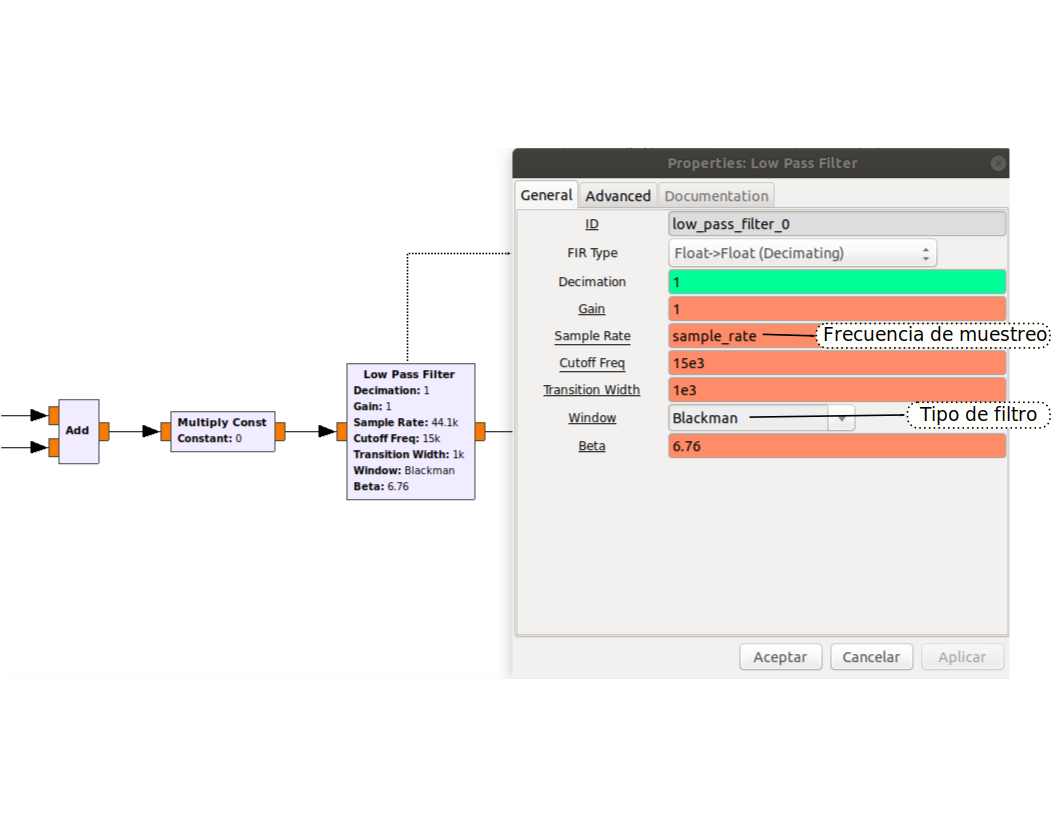
\includegraphics[width=\textwidth]{parte3/lab14/pdf/Lab14_5.pdf}
\end{figure}


\end{frame}
%---------------------------------

\begin{frame}{Desarrollo del diagrama en GNU Radio}

Ahora es necesario realizar la modulación de la señal en FM para ello se configuró el bloque WBFM Transmit.

\begin{figure}[H]
\centering
\vspace{-3mm}
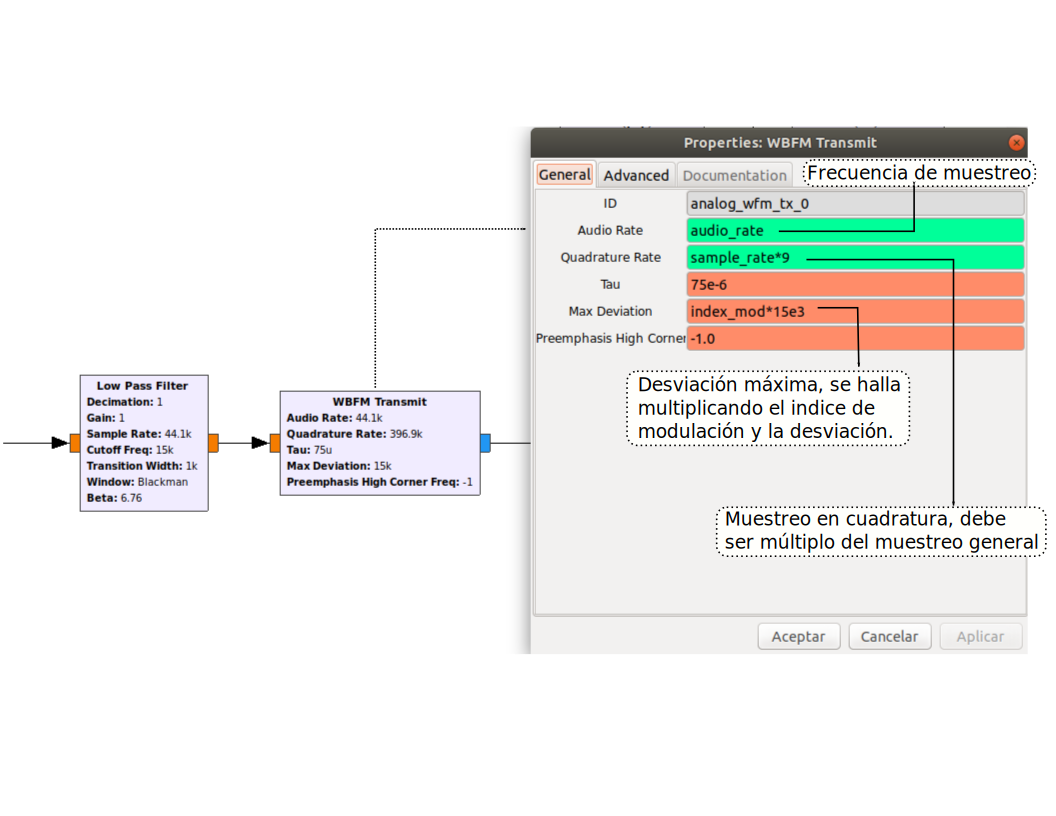
\includegraphics[width=\textwidth]{parte3/lab14/pdf/Lab14_6.pdf}
\end{figure}


\end{frame}
%---------------------------------

\begin{frame}{Desarrollo del diagrama en GNU Radio}

Antes de transmitir se realiza un re-muestreo a una frecuencia que permita a la tarjeta enviar el audio sin ningún problema.

\begin{figure}[H]
\centering
\vspace{-3mm}
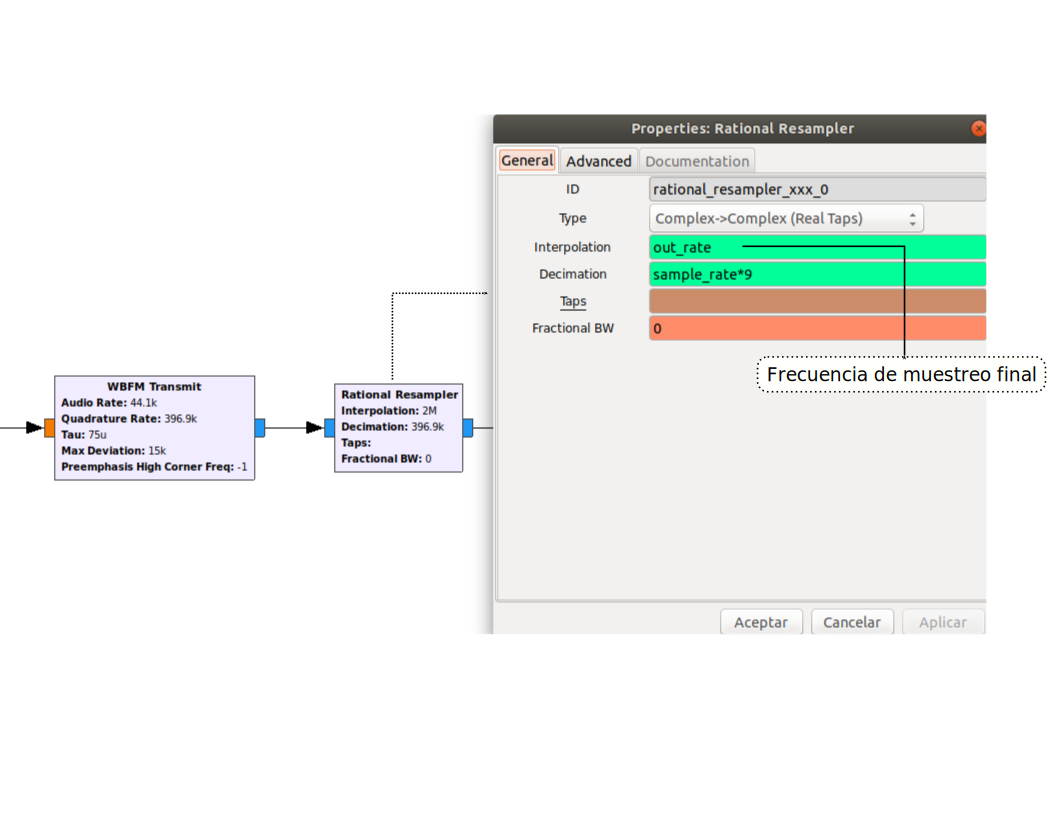
\includegraphics[width=\textwidth]{parte3/lab14/pdf/Lab14_7.pdf}
\end{figure}


\end{frame}
%---------------------------------

\begin{frame}{Desarrollo del diagrama en GNU Radio}

Finalmente se realiza la transmisión de la señal utilizando el bloque Osmocom Sink.

\begin{figure}[H]
\centering
\vspace{-3mm}
\includegraphics[width=\textwidth]{parte3/lab14/pdf/Lab14_8.pdf}
\end{figure}

\end{frame}
%---------------------------------

\begin{frame}{Interfaz gráfica}

La interfaz gráfica está compuesta por 3 páginas diferentes: la primera de ellas consiste en la transmisión final en términos de frecuencia, la segunda permite ver en la señal a transmitir en términos del tiempo y la tercera muestra la información entrante en términos de frecuencia como se puede observar a continuación:

\end{frame}
%---------------------------------

\begin{frame}{Interfaz gráfica}

\begin{figure}[H]
\centering
\vspace{-3mm}
\includegraphics[width=0.9\textwidth]{parte3/lab14/pdf/Lab14_9.pdf}
\end{figure}

\end{frame}
%---------------------------------

\begin{frame}{Interfaz gráfica}

\begin{figure}[H]
\centering
\vspace{-3mm}
\includegraphics[width=0.9\textwidth]{parte3/lab14/pdf/Lab14_10.pdf}
\end{figure}

\end{frame}
%---------------------------------

\begin{frame}{Interfaz gráfica}

\begin{figure}[H]
\centering
\vspace{-3mm}
\includegraphics[width=0.9\textwidth]{parte3/lab14/pdf/Lab14_11.pdf}
\end{figure}

\end{frame}
%---------------------------------   %Cambiar nombre - sobra SDR

%///////////////////////////////////////////////////////////////

\subsection{Lab16: Receptor AM}

%*********************
\begin{frame}{}

\pgfdeclareimage[width=\paperwidth,height=\paperheight]{bg}{imagenes/fondo_lab}
\setbeamertemplate{background}{\pgfuseimage{bg}}

\bfseries{\textrm{\LARGE Lab16\\ \Large Receptor AM}}
\raggedright
\end{frame}
%*********************


%///////////////////////////////////////////////////////////////

\subsection{Lab16: Transmisor AM}

%*********************
\begin{frame}{}

\pgfdeclareimage[width=\paperwidth,height=\paperheight]{bg}{imagenes/fondo_lab}
\setbeamertemplate{background}{\pgfuseimage{bg}}

\bfseries{\textrm{\LARGE Lab16\\ \Large Transmisor AM}}
\raggedright
\end{frame}
%*********************

\begin{frame}{Modulación de amplitud IQ}

\pgfdeclareimage[width=\paperwidth,height=\paperheight]{bg}{imagenes/fondo3}
\setbeamertemplate{background}{\pgfuseimage{bg}}

La modulación de amplitud (AM) funciona mediante la variación de la amplitud de la señal transmitida de alta frecuencia que varía en proporción con una señal que por naturaleza es de baja frecuencia. La señal de baja frecuencia es la información que se desea transmitir también llamada señal moduladora, usualmente se encuentra en el orden de los KHz y la señal de frecuencia alta se le llama portadora usualmente en el orden de los MHz. \\
\vspace{2mm}
Es una modulación digital que transmite dos mensajes independientes y está conformado por dos canales ortogonales $i(t)$ y $q(t)$ que pueden ser transmitidos simultáneamente. \\ \vspace{2mm}  
El canal $i(t)$ es la señal moduladora (entrada) que contiene la información y es la parte real para la transmisión, el canal $q(t)$ es la señal portadora que debe estar desfasada 90$^{\circ}$ de la señal moduladora y es la parte imaginaria para la transmisión\cite{Lecture9}.  




\end{frame}
%---------------------------------

\begin{frame}{Modulación de amplitud IQ}
\begin{wrapfigure}{l}{0.5\linewidth}
    \centering
    \includegraphics[width=0.5\textwidth]{parte3/lab15/pdf/lab15_1.pdf}
\end{wrapfigure}


Matemáticamente se expresa: \\\vspace{3mm}
\centering{
$i_t (t)=i(t)cos(2\pi f_0 t + 0^{\circ})$ \\ \vspace{2mm}
$q_t (t)=q(t)cos(2\pi f_0 t + 90^{\circ})=q(t)sin(2\pi f_0 t)$\\ \vspace{2mm}
$y_t (t)= \sqrt{i^{2} (t)+q^{2}(t)}cos(2\pi f_0 t + \theta(t))$\\ \vspace{2mm}
$\theta(t)=tan^{-1}\frac{q(t)}{i(t)}$\\\vspace{2mm}
$-180<\theta<180^{\circ}$\\ \vspace{2mm}}

\end{frame}
%---------------------------------

\begin{frame}{Modulación de amplitud IQ}

\begin{figure}[H]
\centering
\vspace{-3mm}
\includegraphics[width=\textwidth]{parte3/lab15/pdf/lab15_2.pdf}
\end{figure}

\end{frame}
%---------------------------------

\begin{frame}{Modulación de amplitud IQ}

\begin{figure}[H]
\centering
\vspace{-3mm}
\includegraphics[width=\textwidth]{parte3/lab15/pdf/lab15_3.pdf}
\end{figure}

\end{frame}
%---------------------------------

\begin{frame}{Modulación de amplitud IQ}

\begin{figure}[H]
\centering
\vspace{-3mm}
\includegraphics[width=.7\textwidth]{parte3/lab15/pdf/lab15_4.pdf}
\end{figure}

\end{frame}
%---------------------------------

\begin{frame}{Modulación de amplitud IQ}


El resultado de la modulación (señal modulada) no se puede observar en el dominio del tiempo ni de la frecuencia ya que el proceso de mezclado entre la señal portadora y moduladora se hace directamente con el HackRF, pero sí se puede observar el resultado de la unión entre la parte real e imaginaria (señal moduladora y portadora).  La frecuencia utilizada para mirar la señal en el dominio de la frecuencia (FFT) y el diagrama de cascada (espectrograma) es la sintonizada en el radio.

\end{frame}
%---------------------------------

\begin{frame}{Resultado}

\begin{figure}[H]
\centering
\vspace{-3mm}
\includegraphics[width=\textwidth]{parte3/lab15/pdf/lab15_5.pdf}
\end{figure}

\end{frame}
%---------------------------------

%///////////////////////////////////////////////////////////////


